\documentclass{article} % For LaTeX2e
\usepackage{iclr2021_conference,times}
\usepackage{graphicx,amsmath,amsthm}
\usepackage{showlabels}
\usepackage{iclr2021_extras}
\usepackage{subcaption}

% Optional math commands from https://github.com/goodfeli/dlbook_notation.
%%%% NEW MATH DEFINITIONS %%%%%

\usepackage{amsmath,amsfonts,bm}

% Mark sections of captions for referring to divisions of figures
\newcommand{\figleft}{{\em (Left)}}
\newcommand{\figcenter}{{\em (Center)}}
\newcommand{\figright}{{\em (Right)}}
\newcommand{\figtop}{{\em (Top)}}
\newcommand{\figbottom}{{\em (Bottom)}}
\newcommand{\captiona}{{\em (a)}}
\newcommand{\captionb}{{\em (b)}}
\newcommand{\captionc}{{\em (c)}}
\newcommand{\captiond}{{\em (d)}}

% Highlight a newly defined term
\newcommand{\newterm}[1]{{\bf #1}}


% Figure reference, lower-case.
\def\figref#1{figure~\ref{#1}}
% Figure reference, capital. For start of sentence
\def\Figref#1{Figure~\ref{#1}}
\def\twofigref#1#2{figures \ref{#1} and \ref{#2}}
\def\quadfigref#1#2#3#4{figures \ref{#1}, \ref{#2}, \ref{#3} and \ref{#4}}
% Section reference, lower-case.
\def\secref#1{section~\ref{#1}}
% Section reference, capital.
\def\Secref#1{Section~\ref{#1}}
% Reference to two sections.
\def\twosecrefs#1#2{sections \ref{#1} and \ref{#2}}
% Reference to three sections.
\def\secrefs#1#2#3{sections \ref{#1}, \ref{#2} and \ref{#3}}
% Reference to an equation, lower-case.
\def\eqref#1{equation~\ref{#1}}
% Reference to an equation, upper case
\def\Eqref#1{Equation~\ref{#1}}
% A raw reference to an equation---avoid using if possible
\def\plaineqref#1{\ref{#1}}
% Reference to a chapter, lower-case.
\def\chapref#1{chapter~\ref{#1}}
% Reference to an equation, upper case.
\def\Chapref#1{Chapter~\ref{#1}}
% Reference to a range of chapters
\def\rangechapref#1#2{chapters\ref{#1}--\ref{#2}}
% Reference to an algorithm, lower-case.
\def\algref#1{algorithm~\ref{#1}}
% Reference to an algorithm, upper case.
\def\Algref#1{Algorithm~\ref{#1}}
\def\twoalgref#1#2{algorithms \ref{#1} and \ref{#2}}
\def\Twoalgref#1#2{Algorithms \ref{#1} and \ref{#2}}
% Reference to a part, lower case
\def\partref#1{part~\ref{#1}}
% Reference to a part, upper case
\def\Partref#1{Part~\ref{#1}}
\def\twopartref#1#2{parts \ref{#1} and \ref{#2}}

\def\ceil#1{\lceil #1 \rceil}
\def\floor#1{\lfloor #1 \rfloor}
\def\1{\bm{1}}
\newcommand{\train}{\mathcal{D}}
\newcommand{\valid}{\mathcal{D_{\mathrm{valid}}}}
\newcommand{\test}{\mathcal{D_{\mathrm{test}}}}

\def\eps{{\epsilon}}


% Random variables
\def\reta{{\textnormal{$\eta$}}}
\def\ra{{\textnormal{a}}}
\def\rb{{\textnormal{b}}}
\def\rc{{\textnormal{c}}}
\def\rd{{\textnormal{d}}}
\def\re{{\textnormal{e}}}
\def\rf{{\textnormal{f}}}
\def\rg{{\textnormal{g}}}
\def\rh{{\textnormal{h}}}
\def\ri{{\textnormal{i}}}
\def\rj{{\textnormal{j}}}
\def\rk{{\textnormal{k}}}
\def\rl{{\textnormal{l}}}
% rm is already a command, just don't name any random variables m
\def\rn{{\textnormal{n}}}
\def\ro{{\textnormal{o}}}
\def\rp{{\textnormal{p}}}
\def\rq{{\textnormal{q}}}
\def\rr{{\textnormal{r}}}
\def\rs{{\textnormal{s}}}
\def\rt{{\textnormal{t}}}
\def\ru{{\textnormal{u}}}
\def\rv{{\textnormal{v}}}
\def\rw{{\textnormal{w}}}
\def\rx{{\textnormal{x}}}
\def\ry{{\textnormal{y}}}
\def\rz{{\textnormal{z}}}

% Random vectors
\def\rvepsilon{{\mathbf{\epsilon}}}
\def\rvtheta{{\mathbf{\theta}}}
\def\rva{{\mathbf{a}}}
\def\rvb{{\mathbf{b}}}
\def\rvc{{\mathbf{c}}}
\def\rvd{{\mathbf{d}}}
\def\rve{{\mathbf{e}}}
\def\rvf{{\mathbf{f}}}
\def\rvg{{\mathbf{g}}}
\def\rvh{{\mathbf{h}}}
\def\rvu{{\mathbf{i}}}
\def\rvj{{\mathbf{j}}}
\def\rvk{{\mathbf{k}}}
\def\rvl{{\mathbf{l}}}
\def\rvm{{\mathbf{m}}}
\def\rvn{{\mathbf{n}}}
\def\rvo{{\mathbf{o}}}
\def\rvp{{\mathbf{p}}}
\def\rvq{{\mathbf{q}}}
\def\rvr{{\mathbf{r}}}
\def\rvs{{\mathbf{s}}}
\def\rvt{{\mathbf{t}}}
\def\rvu{{\mathbf{u}}}
\def\rvv{{\mathbf{v}}}
\def\rvw{{\mathbf{w}}}
\def\rvx{{\mathbf{x}}}
\def\rvy{{\mathbf{y}}}
\def\rvz{{\mathbf{z}}}

% Elements of random vectors
\def\erva{{\textnormal{a}}}
\def\ervb{{\textnormal{b}}}
\def\ervc{{\textnormal{c}}}
\def\ervd{{\textnormal{d}}}
\def\erve{{\textnormal{e}}}
\def\ervf{{\textnormal{f}}}
\def\ervg{{\textnormal{g}}}
\def\ervh{{\textnormal{h}}}
\def\ervi{{\textnormal{i}}}
\def\ervj{{\textnormal{j}}}
\def\ervk{{\textnormal{k}}}
\def\ervl{{\textnormal{l}}}
\def\ervm{{\textnormal{m}}}
\def\ervn{{\textnormal{n}}}
\def\ervo{{\textnormal{o}}}
\def\ervp{{\textnormal{p}}}
\def\ervq{{\textnormal{q}}}
\def\ervr{{\textnormal{r}}}
\def\ervs{{\textnormal{s}}}
\def\ervt{{\textnormal{t}}}
\def\ervu{{\textnormal{u}}}
\def\ervv{{\textnormal{v}}}
\def\ervw{{\textnormal{w}}}
\def\ervx{{\textnormal{x}}}
\def\ervy{{\textnormal{y}}}
\def\ervz{{\textnormal{z}}}

% Random matrices
\def\rmA{{\mathbf{A}}}
\def\rmB{{\mathbf{B}}}
\def\rmC{{\mathbf{C}}}
\def\rmD{{\mathbf{D}}}
\def\rmE{{\mathbf{E}}}
\def\rmF{{\mathbf{F}}}
\def\rmG{{\mathbf{G}}}
\def\rmH{{\mathbf{H}}}
\def\rmI{{\mathbf{I}}}
\def\rmJ{{\mathbf{J}}}
\def\rmK{{\mathbf{K}}}
\def\rmL{{\mathbf{L}}}
\def\rmM{{\mathbf{M}}}
\def\rmN{{\mathbf{N}}}
\def\rmO{{\mathbf{O}}}
\def\rmP{{\mathbf{P}}}
\def\rmQ{{\mathbf{Q}}}
\def\rmR{{\mathbf{R}}}
\def\rmS{{\mathbf{S}}}
\def\rmT{{\mathbf{T}}}
\def\rmU{{\mathbf{U}}}
\def\rmV{{\mathbf{V}}}
\def\rmW{{\mathbf{W}}}
\def\rmX{{\mathbf{X}}}
\def\rmY{{\mathbf{Y}}}
\def\rmZ{{\mathbf{Z}}}

% Elements of random matrices
\def\ermA{{\textnormal{A}}}
\def\ermB{{\textnormal{B}}}
\def\ermC{{\textnormal{C}}}
\def\ermD{{\textnormal{D}}}
\def\ermE{{\textnormal{E}}}
\def\ermF{{\textnormal{F}}}
\def\ermG{{\textnormal{G}}}
\def\ermH{{\textnormal{H}}}
\def\ermI{{\textnormal{I}}}
\def\ermJ{{\textnormal{J}}}
\def\ermK{{\textnormal{K}}}
\def\ermL{{\textnormal{L}}}
\def\ermM{{\textnormal{M}}}
\def\ermN{{\textnormal{N}}}
\def\ermO{{\textnormal{O}}}
\def\ermP{{\textnormal{P}}}
\def\ermQ{{\textnormal{Q}}}
\def\ermR{{\textnormal{R}}}
\def\ermS{{\textnormal{S}}}
\def\ermT{{\textnormal{T}}}
\def\ermU{{\textnormal{U}}}
\def\ermV{{\textnormal{V}}}
\def\ermW{{\textnormal{W}}}
\def\ermX{{\textnormal{X}}}
\def\ermY{{\textnormal{Y}}}
\def\ermZ{{\textnormal{Z}}}

% Vectors
\def\vzero{{\bm{0}}}
\def\vone{{\bm{1}}}
\def\vmu{{\bm{\mu}}}
\def\vtheta{{\bm{\theta}}}
\def\va{{\bm{a}}}
\def\vb{{\bm{b}}}
\def\vc{{\bm{c}}}
\def\vd{{\bm{d}}}
\def\ve{{\bm{e}}}
\def\vf{{\bm{f}}}
\def\vg{{\bm{g}}}
\def\vh{{\bm{h}}}
\def\vi{{\bm{i}}}
\def\vj{{\bm{j}}}
\def\vk{{\bm{k}}}
\def\vl{{\bm{l}}}
\def\vm{{\bm{m}}}
\def\vn{{\bm{n}}}
\def\vo{{\bm{o}}}
\def\vp{{\bm{p}}}
\def\vq{{\bm{q}}}
\def\vr{{\bm{r}}}
\def\vs{{\bm{s}}}
\def\vt{{\bm{t}}}
\def\vu{{\bm{u}}}
\def\vv{{\bm{v}}}
\def\vw{{\bm{w}}}
\def\vx{{\bm{x}}}
\def\vy{{\bm{y}}}
\def\vz{{\bm{z}}}

% Elements of vectors
\def\evalpha{{\alpha}}
\def\evbeta{{\beta}}
\def\evepsilon{{\epsilon}}
\def\evlambda{{\lambda}}
\def\evomega{{\omega}}
\def\evmu{{\mu}}
\def\evpsi{{\psi}}
\def\evsigma{{\sigma}}
\def\evtheta{{\theta}}
\def\eva{{a}}
\def\evb{{b}}
\def\evc{{c}}
\def\evd{{d}}
\def\eve{{e}}
\def\evf{{f}}
\def\evg{{g}}
\def\evh{{h}}
\def\evi{{i}}
\def\evj{{j}}
\def\evk{{k}}
\def\evl{{l}}
\def\evm{{m}}
\def\evn{{n}}
\def\evo{{o}}
\def\evp{{p}}
\def\evq{{q}}
\def\evr{{r}}
\def\evs{{s}}
\def\evt{{t}}
\def\evu{{u}}
\def\evv{{v}}
\def\evw{{w}}
\def\evx{{x}}
\def\evy{{y}}
\def\evz{{z}}

% Matrix
\def\mA{{\bm{A}}}
\def\mB{{\bm{B}}}
\def\mC{{\bm{C}}}
\def\mD{{\bm{D}}}
\def\mE{{\bm{E}}}
\def\mF{{\bm{F}}}
\def\mG{{\bm{G}}}
\def\mH{{\bm{H}}}
\def\mI{{\bm{I}}}
\def\mJ{{\bm{J}}}
\def\mK{{\bm{K}}}
\def\mL{{\bm{L}}}
\def\mM{{\bm{M}}}
\def\mN{{\bm{N}}}
\def\mO{{\bm{O}}}
\def\mP{{\bm{P}}}
\def\mQ{{\bm{Q}}}
\def\mR{{\bm{R}}}
\def\mS{{\bm{S}}}
\def\mT{{\bm{T}}}
\def\mU{{\bm{U}}}
\def\mV{{\bm{V}}}
\def\mW{{\bm{W}}}
\def\mX{{\bm{X}}}
\def\mY{{\bm{Y}}}
\def\mZ{{\bm{Z}}}
\def\mBeta{{\bm{\beta}}}
\def\mPhi{{\bm{\Phi}}}
\def\mLambda{{\bm{\Lambda}}}
\def\mSigma{{\bm{\Sigma}}}

% Tensor
\DeclareMathAlphabet{\mathsfit}{\encodingdefault}{\sfdefault}{m}{sl}
\SetMathAlphabet{\mathsfit}{bold}{\encodingdefault}{\sfdefault}{bx}{n}
\newcommand{\tens}[1]{\bm{\mathsfit{#1}}}
\def\tA{{\tens{A}}}
\def\tB{{\tens{B}}}
\def\tC{{\tens{C}}}
\def\tD{{\tens{D}}}
\def\tE{{\tens{E}}}
\def\tF{{\tens{F}}}
\def\tG{{\tens{G}}}
\def\tH{{\tens{H}}}
\def\tI{{\tens{I}}}
\def\tJ{{\tens{J}}}
\def\tK{{\tens{K}}}
\def\tL{{\tens{L}}}
\def\tM{{\tens{M}}}
\def\tN{{\tens{N}}}
\def\tO{{\tens{O}}}
\def\tP{{\tens{P}}}
\def\tQ{{\tens{Q}}}
\def\tR{{\tens{R}}}
\def\tS{{\tens{S}}}
\def\tT{{\tens{T}}}
\def\tU{{\tens{U}}}
\def\tV{{\tens{V}}}
\def\tW{{\tens{W}}}
\def\tX{{\tens{X}}}
\def\tY{{\tens{Y}}}
\def\tZ{{\tens{Z}}}


% Graph
\def\gA{{\mathcal{A}}}
\def\gB{{\mathcal{B}}}
\def\gC{{\mathcal{C}}}
\def\gD{{\mathcal{D}}}
\def\gE{{\mathcal{E}}}
\def\gF{{\mathcal{F}}}
\def\gG{{\mathcal{G}}}
\def\gH{{\mathcal{H}}}
\def\gI{{\mathcal{I}}}
\def\gJ{{\mathcal{J}}}
\def\gK{{\mathcal{K}}}
\def\gL{{\mathcal{L}}}
\def\gM{{\mathcal{M}}}
\def\gN{{\mathcal{N}}}
\def\gO{{\mathcal{O}}}
\def\gP{{\mathcal{P}}}
\def\gQ{{\mathcal{Q}}}
\def\gR{{\mathcal{R}}}
\def\gS{{\mathcal{S}}}
\def\gT{{\mathcal{T}}}
\def\gU{{\mathcal{U}}}
\def\gV{{\mathcal{V}}}
\def\gW{{\mathcal{W}}}
\def\gX{{\mathcal{X}}}
\def\gY{{\mathcal{Y}}}
\def\gZ{{\mathcal{Z}}}

% Sets
\def\sA{{\mathbb{A}}}
\def\sB{{\mathbb{B}}}
\def\sC{{\mathbb{C}}}
\def\sD{{\mathbb{D}}}
% Don't use a set called E, because this would be the same as our symbol
% for expectation.
\def\sF{{\mathbb{F}}}
\def\sG{{\mathbb{G}}}
\def\sH{{\mathbb{H}}}
\def\sI{{\mathbb{I}}}
\def\sJ{{\mathbb{J}}}
\def\sK{{\mathbb{K}}}
\def\sL{{\mathbb{L}}}
\def\sM{{\mathbb{M}}}
\def\sN{{\mathbb{N}}}
\def\sO{{\mathbb{O}}}
\def\sP{{\mathbb{P}}}
\def\sQ{{\mathbb{Q}}}
\def\sR{{\mathbb{R}}}
\def\sS{{\mathbb{S}}}
\def\sT{{\mathbb{T}}}
\def\sU{{\mathbb{U}}}
\def\sV{{\mathbb{V}}}
\def\sW{{\mathbb{W}}}
\def\sX{{\mathbb{X}}}
\def\sY{{\mathbb{Y}}}
\def\sZ{{\mathbb{Z}}}

% Entries of a matrix
\def\emLambda{{\Lambda}}
\def\emA{{A}}
\def\emB{{B}}
\def\emC{{C}}
\def\emD{{D}}
\def\emE{{E}}
\def\emF{{F}}
\def\emG{{G}}
\def\emH{{H}}
\def\emI{{I}}
\def\emJ{{J}}
\def\emK{{K}}
\def\emL{{L}}
\def\emM{{M}}
\def\emN{{N}}
\def\emO{{O}}
\def\emP{{P}}
\def\emQ{{Q}}
\def\emR{{R}}
\def\emS{{S}}
\def\emT{{T}}
\def\emU{{U}}
\def\emV{{V}}
\def\emW{{W}}
\def\emX{{X}}
\def\emY{{Y}}
\def\emZ{{Z}}
\def\emSigma{{\Sigma}}

% entries of a tensor
% Same font as tensor, without \bm wrapper
\newcommand{\etens}[1]{\mathsfit{#1}}
\def\etLambda{{\etens{\Lambda}}}
\def\etA{{\etens{A}}}
\def\etB{{\etens{B}}}
\def\etC{{\etens{C}}}
\def\etD{{\etens{D}}}
\def\etE{{\etens{E}}}
\def\etF{{\etens{F}}}
\def\etG{{\etens{G}}}
\def\etH{{\etens{H}}}
\def\etI{{\etens{I}}}
\def\etJ{{\etens{J}}}
\def\etK{{\etens{K}}}
\def\etL{{\etens{L}}}
\def\etM{{\etens{M}}}
\def\etN{{\etens{N}}}
\def\etO{{\etens{O}}}
\def\etP{{\etens{P}}}
\def\etQ{{\etens{Q}}}
\def\etR{{\etens{R}}}
\def\etS{{\etens{S}}}
\def\etT{{\etens{T}}}
\def\etU{{\etens{U}}}
\def\etV{{\etens{V}}}
\def\etW{{\etens{W}}}
\def\etX{{\etens{X}}}
\def\etY{{\etens{Y}}}
\def\etZ{{\etens{Z}}}

% The true underlying data generating distribution
\newcommand{\pdata}{p_{\rm{data}}}
% The empirical distribution defined by the training set
\newcommand{\ptrain}{\hat{p}_{\rm{data}}}
\newcommand{\Ptrain}{\hat{P}_{\rm{data}}}
% The model distribution
\newcommand{\pmodel}{p_{\rm{model}}}
\newcommand{\Pmodel}{P_{\rm{model}}}
\newcommand{\ptildemodel}{\tilde{p}_{\rm{model}}}
% Stochastic autoencoder distributions
\newcommand{\pencode}{p_{\rm{encoder}}}
\newcommand{\pdecode}{p_{\rm{decoder}}}
\newcommand{\precons}{p_{\rm{reconstruct}}}

\newcommand{\laplace}{\mathrm{Laplace}} % Laplace distribution

\newcommand{\E}{\mathbb{E}}
\newcommand{\Ls}{\mathcal{L}}
\newcommand{\R}{\mathbb{R}}
\newcommand{\emp}{\tilde{p}}
\newcommand{\lr}{\alpha}
\newcommand{\reg}{\lambda}
\newcommand{\rect}{\mathrm{rectifier}}
\newcommand{\softmax}{\mathrm{softmax}}
\newcommand{\sigmoid}{\sigma}
\newcommand{\softplus}{\zeta}
\newcommand{\KL}{D_{\mathrm{KL}}}
\newcommand{\Var}{\mathrm{Var}}
\newcommand{\standarderror}{\mathrm{SE}}
\newcommand{\Cov}{\mathrm{Cov}}
% Wolfram Mathworld says $L^2$ is for function spaces and $\ell^2$ is for vectors
% But then they seem to use $L^2$ for vectors throughout the site, and so does
% wikipedia.
\newcommand{\normlzero}{L^0}
\newcommand{\normlone}{L^1}
\newcommand{\normltwo}{L^2}
\newcommand{\normlp}{L^p}
\newcommand{\normmax}{L^\infty}

\newcommand{\parents}{Pa} % See usage in notation.tex. Chosen to match Daphne's book.

\DeclareMathOperator*{\argmax}{arg\,max}
\DeclareMathOperator*{\argmin}{arg\,min}

\DeclareMathOperator{\sign}{sign}
\DeclareMathOperator{\Tr}{Tr}
\let\ab\allowbreak


\usepackage{hyperref}
\usepackage{url}


\title{Deep Learning is Singular Learning}

% Authors must not appear in the submitted version. They should be hidden
% as long as the \iclrfinalcopy macro remains commented out below.
% Non-anonymous submissions will be rejected without review.

\author{Antiquus S.~Hippocampus, Natalia Cerebro \& Amelie P. Amygdale \thanks{ Use footnote for providing further information
about author (webpage, alternative address)---\emph{not} for acknowledging
funding agencies.  Funding acknowledgements go at the end of the paper.} \\
Department of Computer Science\\
Cranberry-Lemon University\\
Pittsburgh, PA 15213, USA \\
\texttt{\{hippo,brain,jen\}@cs.cranberry-lemon.edu} \\
\And
Ji Q. Ren \& Yevgeny LeNet \\
Department of Computational Neuroscience \\
University of the Witwatersrand \\
Joburg, South Africa \\
\texttt{\{robot,net\}@wits.ac.za} \\
\AND
Coauthor \\
Affiliation \\
Address \\
\texttt{email}
}

\RequirePackage{algorithm}
\RequirePackage{algorithmic}

% The \author macro works with any number of authors. There are two commands
% used to separate the names and addresses of multiple authors: \And and \AND.
%
% Using \And between authors leaves it to \LaTeX{} to determine where to break
% the lines. Using \AND forces a linebreak at that point. So, if \LaTeX{}
% puts 3 of 4 authors names on the first line, and the last on the second
% line, try using \AND instead of \And before the third author name.

\def\be{\begin{equation}}
\def\ee{\end{equation}}
\newcommand{\fix}{\marginpar{FIX}}
\newcommand{\new}{\marginpar{NEW}}
\def\l{\,|\,}
\def\lto{\longrightarrow}

%\iclrfinalcopy % Uncomment for camera-ready version, but NOT for submission.
\begin{document}


\maketitle

\begin{abstract}
Despite its potential for addressing fundamental mysteries in deep learning, singular learning theory appears to have made little inroads into the developing canon of deep learning theory. In this note we present an invitation to key ideas of singular learning theory via a mix of theory and simple experiments, in the hope of making the topic accessible to a wider audience. 
\end{abstract}

\section{Introduction}

It has been understood for close to twenty years that neural networks are singular statistical models \cite{amari_learning_2003, watanabe_almost_2007}. This means that the set of weights with zero loss form a real analytic variety which fails to be an analytic manifold because of the presence of singularities. It has been shown by Sumio Watanabe that the geometry of these singularities control quantities of interest in statistical learning theory such as the Bayes generalisation error. The study of singular models, also known as singular learning theory \citep{watanabe_algebraic_2009}, requires very different tools from the study of regular statistical models. The breadth of knowledge demanded by singular learning theory -- Bayesian statistics, empirical processes and algebraic geometry -- is rewarded with profound and surprising results which reveal singular models are different from regular models in practically important ways.

In order to illustrate the relevance of singular learning theory to deep learning, the paper consists of several sections each of which illustrates one key take-away idea:

\textbf{Neural networks are singular models.} (Section \ref{section:nn_singular}). A many-layered neural network statistical model is non-identifiable and has degenerate Fisher information matrix \emph{at every point of the parameter space}. Classical tools from statistical inference are hence inappropriate for deep neural networks, e.g., one should not ``divide" by the determinant of the Hessian in deep learning. 

\textbf{The real log canonical threshold (RLCT) is the correct way to count the effective number of parameters in a deep neural network.} (Section \ref{section:no_flat_minima}). 
    To every (model, truth, prior) triplet is associated a birational invariant known as the real log canonical threshold (RLCT). The RLCT can be understood as the number of normal directions to the set of true parameters. We will explain why this matters much more than the curvature of those directions (as measured for example by eigenvalues of the Hessian), laying bare some of the confusion over ``flat'' minima in deep learning 

\textbf{For singular models, Bayes predictive distribution is superior to MAP and MLE} (Section \ref{section:gen_error}). In regular statistical models, MAP, MLE, and the Bayes predictive distribution share the same leading term in the asymptotic expansion of the Kullback-Leibler generalization error. This is not so in singular models. We illustrate in our experiments that even ``being Bayesian'' in just the final layers improves generalization over MAP. Our experiments further confirm that the Laplace approximations of the predictive distribution is indeed not appropriate in deep learning.

\textbf{The complexity of a singularity is inversely proportional to the RLCT} (Section \ref{section:simple_func}). In singular models the RLCT depends on the (model, truth, prior) triple whereas in regular models it depends only on the (model, prior) pair.
     %under a hypothesis of realizability 
     We verify this experimentally with a simple family of ReLU networks. Furthermore we empirically observe that the complexity of a singularity is inversely proportional to the RLCT.


\section{Singular Learning Theory}

In classical learning theory, generalization is explained by measures of capacity such as the $l_2$ norm, Radamacher complexity, and VC dimension \citep{bousquet2003introduction}. It has become clear however that these measures are unable to account for the empirical success of deep neural networks \citep{zhang_understanding_2017}. 
%Rethinking generalization will likely require devising capacity measures suitable to the peculiarities of deep learning, e.g. non-identifiability and degenerate Fisher information matrix. 
To understand why classical measures of capacity fail to say anything meaningful about deep neural networks (DNN), it is important to distinguish between two different types of statistical models. Suppose we are interested in estimating the true (unknown) conditional distribution $q(y|x)$ with a class of models $\{p(y|x,w): w \in W\}$ where $W \subset \mathbb R^d$ is the parameter space. Let 
$$
W_0 = \{w \in W: p(y|x,w)=q(y|x)\}
$$
 be the set of true parameters. We say the model is \textit{identifiable} if $W_0$ is a singleton. Let $q(x)$ be the distribution of $x$. The Fisher information matrix associated with the model $\{p(y|x,w)\}$ is the matrix-valued function on $W$ defined by
 \begin{equation*}
 I(w)_{ij} = \int\!\int \frac{\partial}{\partial w_i}[ \log p(y|x,w) ] \frac{\partial}{\partial w_j}[ \log p(y|x,w) ] q(y|x) q(x) dx dy,
 \label{eq:FIM}
 \end{equation*}
if this integral is finite. 
Following the conventions in \cite{watanabe_algebraic_2009}, we have the following bifurcation of statistical models:
\begin{definition}
A statistical model $p(y|x,w)$ is called \textbf{regular} if it is 1) identifiable and 2) has positive-definite Fisher information matrix. A statistical model is called \textbf{strictly singular} if it is not regular. 
%{\cite[Theorem 7.2]{watanabe_algebraic_2009}}.
\end{definition}

% \begin{definition}[Singular model]
% A singular statistical model is either a regular model or a strictly singular model. 
% \end{definition}

Let  $\varphi(w)$ be a prior on the model parameters $w$.
To every model-truth-prior triplet, we can associate the zeta function
\begin{equation}
\zeta(z) = \int K(w)^z \varphi(w) \,dw, \quad z \in \mathbb C,
\end{equation} 
where $K(w)$ is the Kullback-Leibler divergence between the model $p(y|x,w)$ and the true distribution $q(y|x)$:
\begin{equation}
    K(w) := \int \!\int q(y|x) \log \frac{ q(y|x) }{ p(y|x,w) } q(x) \,dx \,dy.
\end{equation}
Then to every triplet of model-truth-prior, we can associate the following central quantity of singular learning theory:

\begin{definition}[Real log canonical threshold (RLCT)]
For a model-truth-prior triplet $(p(y|x,w),q(y|x),\varphi)$, let $-\lambda$ be the maximum pole of the corresponding zeta function. We call $\lambda$ the real log canonical threshold of the model-truth-prior triplet.
\label{def:RLCT}
\end{definition}

By {\citet[Theorem 6.4]{watanabe_algebraic_2009}}, the RLCT is equal to $d/2$ in regular statistical models and bounded above by $d/2$ in strictly singular models if \textit{realizability} holds:
 \begin{definition}
	We say $q(y|x)$ is \textbf{realizable} by the model class $\{p(y|x,w)\}$ if $W_0$ is non-empty.
\end{definition}
The condition of realizability is critical to standard results in singular learning theory. Modifications to the theory are needed in the case that $q(y|x)$ is not realizable, see the more general condition called relatively finite variance in \citet{watanabe_mathematical_2018}.

% The work of Sumio Watanabe on singular learning theory \cite{watanabe_algebraic_2009} suggests that the \textit{real log canonical threshold} (RLCT) of a deep neural network is suitable for measuring its effective number of parameters (see Section ???). 
\textbf{RLCT plays an important role in model selection}
One of the most accessible results in singular learning theory is the work related to the widely-applicable Bayesian information criterion (WBIC) \citet{watanabe_widely_2013}, which we briefly review here for completeness.
Let $\mathcal D_n =  \{(x_i,y_i)\}_{i=1}^n$ be a dataset of input-output pairs.  
Let $L_n(w)$ be the negative log likelihood
\begin{equation}
L_n(w) = -\frac{1}{n} \sum_{i=1}^n \log p(y_i |x_i, w)
\label{eq:nll}
\end{equation}
The marginal likelihood of a model $\{p(y|x,w): w \in W\}$ is given by
$
p(\mathcal D_n) = \int_W p(\mathcal D_n|w) \varphi(w) \,dw
$
and can be loosely interpreted as the evidence for the model. Between two models, we should prefer the one with higher model evidence.
However, since the marginal likelihood is an intractable integral over the parameter space of the model, one needs to consider some approximation.

Recall that the well-known Bayesian Information Criterion (BIC) derives from an asymptotic approximation of the negative log marginal likelihood, $-\log p(\mathcal D_n)$, using the Laplace approximation, leading to
\[
\operatorname{BIC} = nL_n( w_{mle}) + \frac{d}{2} \log n.
\]
Since we want the marginal likelihood of the data for some given model to be \textit{high}, we want the negative log marginal likelihood to be \textit{low}. Thus when $d$ is extremely large as is the case in deep neural networks, one should almost never adopt a deep network according to the BIC. 
%(aka the log marginal likelihood, aka the free energy). 
% Given two statistical models of a data source, one should choose (all else being equal) the one with higher model evidence. 

However, this argument contains a serious mathematical error: the Laplace approximation used to derive BIC only applies to \emph{regular} statistical models, and deep neural networks are not regular. Deep neural networks are \textit{strictly singular} as we illustrated in Section \ref{section:nn_singular}. 
If we have realizability (along with a few more technical conditions), the correct criterion for both regular and strictly singular models was shown in \citet{watanabe_widely_2013} to be 
\begin{equation}
nL_n(w_0) + \lambda \log n,
\label{logmarginal_rlct}
\end{equation}
where $w_0 \in W_0$ and $\lambda$ is the RLCT. 
Since more complex singularities lead to smaller values of $\lambda$, which we illustrate in Section \ref{section:simple_func}, and deep learning models are highly singular, it is possible for deep neural networks to have high marginal likelihood -- consistent with their empirical success. 

The RLCT is a birational invariant \citep{kollar_birational_1998} that measures the complexity of singularities in the model. Since the complexity of singularities determine most of the interesting properties of a model, the RLCT is a very appealing choice for understanding, say, the generalization behavior in singular models, particularly deep neural networks. Furthermore the RLCT as a capacity measure is theoretically rigorous which most existing capacity measures for deep neural networks cannot claim. While theoretical investigations of a deep network's generalization behavior is an active area of research \cite{neyshabur_exploring_2017}, it is still common practice to work with degenerate Hessians in proposing capacity measures, e.g., \citet{thomas_information_2019}. Another common mistake is to perform the Laplace approximation for singular neural networks. For instance, both \citet{zhang_energyentropy_2018} and  \citet{le_bayesian_2018} have explanations of the generalization error of the full Bayes predictor that relies on the Laplace approximation of the intractable posterior distribution. ???Also discuss the following works \cite{maddox_rethinking_2020}, \cite{gao_degrees_2016}, \cite{sun_lightlike_2020}.???


\section{Neural networks are strictly singular}
\label{section:nn_singular}
Many-layered neural networks are strictly singular. There seems to be only informal acknowledgment of this fact in the deep learning community. For instance the recent work in \citet{pennington_spectrum_2018} deliberately studies the Fisher information matrix of a \textit{single-hidden-layer} neural network. If instead the interest is in a many-layered network, one must work with rather ad-hoc workarounds  \citep{sun2017relative}.  

We first explain how to think about a neural network in the context of singular learning theory. A feedforward network of depth $k$ parametrises a function $f: \mathbb{R}^N \lto \mathbb{R}^M$ of the form
\[
f = A_k \circ \sigma_{k-1} \circ A_{k-1} \cdots \sigma_1 \circ A_1
\]
where the $A_i: \mathbb{R}^{d_i} \lto \mathbb{R}^{d_{i+1}}$ are affine functions and $\sigma_i: \mathbb{R}^{d_{i+1}} \lto \mathbb{R}^{d_{i+1}}$ is coordinate-wise some fixed nonlinearity $\sigma: \mathbb{R} \lto \mathbb{R}$. Let $W$ be a compact subspace of the space $\mathbb{R}^D$ containing the origin, where $\mathbb{R}^D$ is the space of sequences affine functions $(A_i)_{i=1}^k$ with coordinates denoted $w_1,\ldots,w_D$, so that $f$ may be viewed as a function $f: \mathbb{R}^N \times W \lto \mathbb{R}^M$. We define
\begin{equation}
p(y|x,w) = \frac{1}{(2 \pi)^{M/2}} \exp\Big(-\tfrac{1}{2} \| y - f(x,w) \|^2 \Big)\,.
\label{eq:gaussian_model_in_w}
\end{equation}
We assume the true distribution is realisable, $q(y|x) = p(y|x,w_0)$ and that a distribution $q(x)$ on $\mathbb{R}^N$ is fixed with respect to which $p(x,y) = p(y|x)q(x)$ and $q(x,y) = q(y|x)q(x)$. Given some prior $\varphi(w)$ on $W$ we may apply singular learning theory to the triplet $(p,q,\varphi)$.

By straightforward calculations we obtain
\begin{gather}
K(w) = \tfrac{1}{2} \int q(x) \| f(x,w) - f(x,w_0) \|^2 dx\\
I(w)_{ij} = \frac{1}{2^{(M-3)/2} \pi^{(M-2)/2}} \int \Big\langle \tfrac{\partial}{\partial w_i} f(x,w), \tfrac{\partial}{\partial w_j} f(x,w) \Big\rangle q(x) dx\label{eq:fisher_relu}
\end{gather}
where $\langle -, - \rangle$ denotes the dot product on $\mathbb{R}^M$. Given $w \in W$ we let $\mathcal{D}(w)$ denote the complement in $\mathbb{R}^N$ of the union over all hidden nodes of the decision boundary at that node (clarify). Since each of these decision boundaries is a hyperplane, $\mathcal{D}(w)$ is a disjoint union of finitely many open chambers. The partial derivative with respect to $\frac{\partial}{\partial w_j}$ of $f: \mathbb{R}^N \times W \lto \mathbb{R}^M$ exists at any point $(x,w)$ with $x \in \mathcal{D}(w)$. We assume that $q(x)$ has been chosen such that this integral exists.

We prove the common feedforward ReLU network has degenerate Fisher information matrix. 

\begin{lemma}\label{lemma:reln} Suppose $\sigma = \operatorname{ReLU}$. For any hidden node in the network with coordinates $(a_k)_k$ for the incoming weights, $(b_i)_i$ for the outgoing weights and $c$ for the bias
\begin{align*}
\Big\{ \sum_k a_{k}\frac{\partial}{\partial a_k} + c \frac{\partial}{\partial c}-\sum_{i} b_i\frac{\partial}{\partial b_i} \Big\} f = 0.
\end{align*}
\end{lemma}
\begin{proof}
Let $e_i$ denote unit vectors and $H(x)=\frac{d}{dx}\operatorname{ReLU}(x)$. Let $u$ and $a$ denote the value of node before and after activation, respectively $u =\sum_k w_k a_{k}^{l-1}+b_{j}^{l}$ and $a_{j}^{l} =\operatorname{ReLU}(u_{j}^{l})$. Then
\begin{align*}
\frac{\partial f}{\partial q_i}&=\frac{\partial y}{\partial u}u_{j}^{l}H(u_{j}^{l})e_{i}\\
\frac{\partial y}{\partial w_{jk}^{l}}&=\frac{\partial y}{\partial u^{l+1}}\frac{\partial u^{l+1}}{\partial w_{jk}^{l}}=\frac{\partial y}{\partial u^{l+1}}\sum_{i=1}^{d_{l+1}}w_{ij}^{l+1}a_{k}^{l-1}H(u_{j}^{l})e_{i}.\\
\frac{\partial y}{\partial b_{j}^{l}}&=\frac{\partial y}{\partial u^{l+1}}\frac{\partial u^{l+1}}{\partial b_{j}^{l}}=\frac{\partial y}{\partial u^{l+1}}\sum_{i=1}^{d_{l+1}}w_{ij}^{l+1}H(u_{j}^{l})e_{i}.
\end{align*}
The claim immediately follows (TODO: fix notation).
\end{proof}

\begin{lemma} If $\sigma = \operatorname{ReLU}$ the matrix $I(w)$ is degenerate at every nonzero point of $W$.
\end{lemma}
\begin{proof}
Let $w \in W$ be given, and choose a hidden node where at least one of the incident weights (or bias) is nonzero. Then Lemma \ref{lemma:reln} gives a nontrivial linear dependence relation $\sum_i \lambda_i \frac{\partial}{\partial w_i} f = 0$ as functions on $\mathbb{R}^N$. The rows of $I(w)$ satisfy the same linear dependence relation.
\end{proof}

The well-known positive scale invariance of ReLU networks is responsible for the linear dependence of Lemma \ref{lemma:reln}, but this is only one source of degeneracy or singularity in ReLU networks. As we show in Section \ref{??} even once this symmetry is ``fixed'' there is additional degeneracy (as measured by the RLCT).

\begin{remark} (cleanup)
e.g. Amari, this lightlike-neuromanifold thing) that make this minimal singularity assumption are just irrelevant to deep learning.
\end{remark}

\section{Volume dimension, effective degrees of freedom, and flatness}
\label{section:no_flat_minima}

\textbf{Volume dimension}. The easiest way to understand the RLCT is as a volume dimension \citep[Theorem 7.1]{watanabe_algebraic_2009}.  Suppose $W_0$ is nonempty, i.e., the true distribution is realizable and that $W \subseteq \mathbb{R}^d$. We consider a special case in which a neighborhood of every point $w_0 \in W_0$ the Kullback-Liebler distance has the following expression in local coordinates
\begin{equation}\label{eq:local_Kw}
K(w) = \sum_{i=1}^{d'} c_i w_i^2,
\end{equation} %This corresponds to a reduced rank regression model, or a neural network with two linear layers and the identity function: $f_w(x) = BAx$ where $B$ and $A$ are matrices of the appropriate size. 
where the coefficients $c_1,\ldots,c_{d'} > 0$ may depend on $w_0$ and $d'$ may be strictly less than $d$. It follows that the set $W_0 \subseteq W$ of true parameters is a regular submanifold of codimension $d'$ (that is, $W_0$ is a manifold of dimension $d - d'$ where $W$ has dimension $d$). Under this hypothesis there are, near each true parameter $w_0 \in W_0$, exactly $d - d'$ directions in which $w_0$ can be varied without changing the model $p(y|x,w)$ and $d'$ directions in which varying the parameters does change the model. In this sense, there are $d'$ \emph{effective parameters} (or \emph{effective degrees of freedom}) near $w_0$. 

This effective dimension near $w_0$ can be computed by an integral. To see this, define the volume of the set of ``almost true'' parameters
%This is not true in general, and it is not true of deep neural networks, but it is true of regular models with $d' = 0$ (the set of true parameters is a set of isolated points) and for singular models such as reduced rank regression with $d' > 0$.
\begin{equation}\label{eq:true_param}
V(t) = \int_{K(w) < t} \varphi(w) dw
\end{equation}
where the integral is restricted to some sufficiently small open neighborhood of $w_0$. As long as the prior $\varphi(w)$ is non-zero on $W_0$ it does not affect the relevant features of the volume, so we may assume $\varphi$ is constant on the region of integration in the first $d'$ directions and normal in the remaining directions, so up to a constant depending only on $d'$ we have
\begin{equation}\label{eq:volume_singular}
V(t) \propto \frac{t^{d'/2}}{\sqrt{c_1 \cdots c_{d'}}}
\end{equation}
and we can extract the exponent of $t$ in this volume in the limit
\be\label{eq:limit_volumedim}
d' = 2 \lim_{t \to 0} \frac{\log\big\{V(at)/V(t)\big\}}{\log(a)}
\ee
for any $a > 0$, $a \neq 1$. The right hand side of (\ref{eq:limit_volumedim}) is the \emph{volume dimension} associated to $K$. 

The function $K(w)$ has the special form (\ref{eq:local_Kw}) locally with $d' = d$ if the statistical model is regular (and realisable) and with $d' < d$ in some singular models such as reduced rank regression (Appendix \ref{??}). While such a local form does not exist for a general singular model (in particular for neural networks) nonetheless under natural conditions Watanabe shows that \citet[Theorem 7.1]{watanabe_algebraic_2009}
\[
V(t) = c t^\lambda + o( t^\lambda)
\]
where $\lambda$ is the RLCT and $c$ is a constant.\footnote{We are assuming that in a sufficiently small neighborhood of $w_0$ the RLCT at $w_0$ is less than or equal to the RLCT at every point in the neighborhood so that the multiplicity $m = 1$, see Section 7.6 of \citep{watanabe_algebraic_2009}.} It follows that the limit on the right hand side of  (\ref{eq:volume_singular}) exists and is equal to $\lambda$. In particular $\lambda = d/2$ in the regular case and $d'/2$ in the more general case of (\ref{eq:local_Kw}) above. In general it is appropriate to think of $2 \lambda$ as a volume dimension, or as the effective number of parameters near $w_0$.\footnote{In general $\lambda$ is a rational number, so it is not straightforward to give a geometric interpretation of why the volume grows as $t^\lambda$. Such an analysis requires an understanding of the resolution of singularities.}

%It can be easily shown in this special case that the RLCT $\lambda = d'/2$. In other words, $2\lambda$ is the effective number of parameters in the model.

\textbf{RLCT and likelihood vs temperature}. Let us assume that our statistical model is of the exponential form  (\ref{eq:gaussian_model_in_w}) and let $D_n = \{ (x_i,y_i) \}_{i=1}^n$ be sampled from the true distribution. The negative log likelihood is
\begin{equation}
L_n(w) = \frac{M}{2} \log(2\pi) + \frac{1}{n} \sum_{i=1}^n \frac{1}{2} \| y_i - f(x_i,w) \|^2\,.
\end{equation}
Given a temperature $T$ consider the quantity $E(T)$ 
\[
E(T) = \mathbb{E}^{1/T}_w\big[nL_n(w) \big] = \mathbb{E}_w^{1/T}\Big[ \tfrac{1}{2} \sum_{i=1}^n \| y_i - f(x_i, w) \|^2 \Big] + \frac{nM}{2} \log(2\pi)\,.
\]
where $p^{1/T}(w|D_n)$ is the Bayesian posterior at temperature $T$ of (\ref{general_posterior}).

Note that when $n$ is large $L_n(w_0) \approx \frac{M}{2} \log(2\pi)$ for any $w_0 \in W_0$ so for $T \approx 0$ the posterior concentrates around the set $W_0$ of true parameters and $E(T) \approx \frac{nM}{2} \log(2\pi)$. Consider the increase $\Delta E = E(T + \Delta T) - E(T)$ corresponding to an increase in temperature $\Delta T$. It can be shown that 
\[
\Delta E \approx \lambda \Delta T
\]
where the reader should see \citep[Corollary 3]{watanabe_widely_2013} for a precise statement. As the temperature increases, samples taken from the tempered posterior are more likely to come from further away from $W_0$ and $E$ will increase. If $\lambda$ is smaller then for a given increase in temperature the quantity $E$ increases less: this is one way to understand why a model with smaller RLCT generalises better from the dataset $D_n$ to the true distribution.\footnote{The relation $\Delta E \approx \lambda \Delta T$ holds for the global RLCT. If the posterior is defined with respect to a prior $\varphi(w)$ which is concentrated around a point $w_0$ with lower point RLCT than any other point in its neighborhood, as above, then the same relation holds for the point RLCT $\lambda$.}

%Hence if $d'_0 < d'_1$ then the model we obtain by integrating near $w_0$ will have an error which increases less quickly with temperature. From the point of view of statistical learning two true parameters with different volume dimensions are not equivalent.

%\textbf{Not all true parameters are created equal} More generally, we can consider a model in which $K(w)$ has the form (\ref{eq:local_Kw})  near each point of $W_0$ but where the codimension $d'$ (and hence the volume dimension) varies from point to point (for instance $W_0$ might be a disjoint union of two regular submanifolds). What are we to make of such a situation? Since two true parameters $w_0, w_1$ with different volume dimensions $d_0' < d_1'$ still determine the same model, the significance of this situation requires explanation.


%We take the point of view that in deep learning it is not meaningful to talk about \emph{points} $w \in W$ as this would suggest an inference procedure of infinite precision. The only ``physically'' meaningful quantities are distributions $\psi(w)$ over $W$ and the associated predictive distributions
%\[
%p^*_\psi(y|x) = \int p(y|x,w) \psi(w) dw\,.
%\]
%While two parameters $w_0, w_1$ with volume dimensions $d'_0, d'_1$ determine the same model, if the predictive distributions $p^*_{\psi_1}(y|x)$ and $p^*_{\psi_2}(y|x)$ are essentially different for $\psi_i$ arbitrarily concentrated around $w_i$ then the two parameters are, in a deeper sense, not equivalent. For example, suppose the statistical model is of exponential form, as with the models defined in Section \ref{??} associated to two-layer ReLU networks. 

%\begin{remark}
%The explanation requires examining local neighborhoods around $w_0$ and $w_1$ with respect to the %\textit{posterior distribution}:
%\begin{equation}
%p(w|\mathcal D_n) \propto \Pi_{i=1}^n p(y_i|x_i,w) \varphi(w)
%\end{equation}
%Namely, we must compare $E_w \displaystyle \1_\mathrm{w \in U(w_0)}$ and $E_w \displaystyle \1_\mathrm{w \in U(w_1)}$ where for random variable $R(w)$
%\begin{equation}
%{\E}_w [R(w)] := \int_W R(w) p(w|\mathcal D_n) \,dw
%\label{eq:E_w}
%\end{equation}
%For any $w^* \in W$, we can write
%$
%E_w \displaystyle \1_\mathrm{w \in U(w^*)} = p(w^*|\mathcal D_n) Z(w^*).
%$
%Watanabe pointed out that the more complicated singularity (smaller RLCT) has higher $Z(w^*)$. Since $d_0' < d_1'$, $w_0$ is the more complicated singularity and we have
%$$
%E_w \displaystyle \1_\mathrm{w \in U(w_0)} > E_w \displaystyle \1_\mathrm{w \in U(w_1)}
%$$
%This is to say that two true parameters may lead to the same model, but could have vastly different behavior if we look at \eqref{eq:E_w} restricted to local neighborhoods of the true parameters. 
%\end{remark}

%We take the point of view that in deep learning it is not meaningful to talk about \emph{points} $w \in W$ as this would suggest an inference procedure of infinite precision. The only ``physically'' meaningful quantities are distributions $\psi(w)$ over $W$ and the associated predictive distributions
%\[
%p^*_\psi(y|x) = \int p(y|x,w) \psi(w) dw\,.
%\]
%While two parameters $w_0, w_1$ with volume dimensions $d'_0, d'_1$ determine the same model, if the predictive distributions $p^*_{\psi_1}(y|x)$ and $p^*_{\psi_2}(y|x)$ are essentially different for $\psi_i$ arbitrarily concentrated around $w_i$ then the two parameters are, in a deeper sense, not equivalent. For example, suppose the statistical model is of exponential form, as with the models defined in Section \ref{??} associated to two-layer ReLU networks. 
%
%Given a fixed dataset $D_n = \{ (x_i,y_i) \}_{i=1}^n$ sampled from the true distribution we consider the expected squared error over the dataset
%\[
%E(T) = \mathbb{E}_w^T\Big[ \sum_{i=1}^n \| y_i - f(x_i, w) \|^2 \Big]
%\]
%where $w$ from the posterior at temperature $T$. This quantity is a random variable, which depends on the dataset $D_n$ the temperature $T$ and the prior $\varphi(w)$ that is placed on the parameters. The temperature controls how finely parameters are distinguished: at high temperature points with high posterior probability are barely distinguishable from points with low probability, and as $T \lto 0$ all the probability concentrates around true parameters. Consider the change $\Delta E = E(T + \Delta T) - E(T)$ resulting from an increase in the temperature. This is a measure of sensitivity of the performance of the predictive distribution to temperature. If our prior $\varphi = \psi_i$ is concentrated near a point $w_i \in W_0$ of volume dimension $d'_i$, then it can be shown that
%\[
%\Delta E \approx d'_i \Delta T
%\]
%Hence if $d'_0 < d'_1$ then the model we obtain by integrating near $w_0$ will have an error which increases less quickly with temperature. From the point of view of statistical learning two true parameters with different volume dimensions are not equivalent.

\textbf{Flatness}. It is folklore in the deep learning community that flatness of minima is related to generalisation \citep{hinton_keeping_1993, hochreiter1997flat} and this claim has been revisited in recent years \citep{chaudhari2019entropy, smith2017bayesian, jastrzkebski2017three, Zhang:2018MolPh.116.3214Z}. In regular models this can be justified using the lower order terms of the asymptotic expansion of the Bayes free energy \citep[\S 3.1]{Balasubramanian:1996cond.mat..1030B} but the argument breaks down in singular models, since for example the Laplace approximation of \cite{Zhang:2018MolPh.116.3214Z} is invalid. The basic point can be understood by a close analysis of the version of the idea in \citep{hochreiter1997flat}. Their measure of entropy compares the volume of the set of parameters with tolerable error $t_0$ (our ``almost true'' parameters) to a standard volume defined without the Kullback-Liebler function
\begin{equation}\label{eq:entropy}
- \log\Big[\frac{V(t_0)}{t_0^{d/2}}\Big] = \frac{d-d'}{2} \log(t_0) + \tfrac{1}{2} \sum_{i=1}^{d} \log c_i\,.
\end{equation}
Hence in the case $d = d'$ the quantity $-\tfrac{1}{2} \sum_i \log(c_i)$ is a measure of the entropy of the set of true parameters near $w_0$, a point made for example in \cite{Zhang:2018MolPh.116.3214Z}. However when $d' < d$ this conception of entropy is inappropriate because of the $d - d'$ directions in which $K(w)$ is flat near $w_0$, which introduce the $t_0$ dependence in (\ref{eq:entropy}).

% Note that in comparing two regular models with parameter space $W \subseteq \mathbb{R}^d$, both of which have volume dimension $d/2$, the Hessian determinant is relevant to compare how the respective volumes of almost true parameters vary with $t$. But in comparing two minimally singular models with Hessian determinants of rank $d', d''$ the behavior of the volume depends much more strongly on the dimensions $d'/2, d''/2$ than it does on the eigenvalues.
% From a theoretical point of view the exponent $d/2$ appears as the leading $O(\log n)$ term in the asymptotic expansion of the Bayes free energy and the Hessian determinant appears in the next $O(1)$ term, where $n$ is the size of a dataset . The upshot of this is that if two regular models have parameter spaces of dimension $d_1 < d_2$ one should prefer the model class of dimension $d_1$ (assuming both can perfectly fit the data) but if $d_1 = d_2$ then it may be appropriate to compare models on the basis of their curvature at the true parameter.

% What kind of space is the set of true parameters of a singular statistical model? In modern mathematics we generally think of spaces as a pair consisting of a topological space $X$ and a sheaf of rings, which for every open subset $U \subseteq X$ picks out a certain class of continuous functions $U \lto \mathbb{R}$. In the theory of smooth or analytic manifolds, for instance, these would be the $C^\infty$ or $C^\omega$ functions, while in algebraic geometry these would be the regular functions. Historically statistical learning theory and machine learning has mostly employed concepts of space from differential geometry, where this sheaf can be safely left implicit: if $X \subseteq \mathbb{R}^D$ is a regular submanifold, the manifold structure on $X$ can be recovered from the \emph{set} $X$ and the manifold structure on $\mathbb{R}^D$. However in algebraic geometry a closed subspace does \emph{not} have an unambiguous structure as a space in its own right:

%\begin{example} The zero locus of $x$ and $x^2$ in $\mathbb{R}^2$ have the same underlying set, but as schemes the former is smooth and has coordinate ring $\mathbb{R}[x,y]/x \cong \mathbb{R}[y]$ while the latter is singular and has coordinate ring $\mathbb{R}[x,y]/x^2$. Singularity vs regularity is \emph{not a property of the set} but the function whose zero locus the set is.
%\end{example}

\section{Generalization}\label{section:gen_error}
In the Bayesian paradigm, prediction proceeds via the so-called Bayes predictive distribution
\begin{equation}
p(y|x, \mathcal D_n) = \int p(y|x,\theta) p(\theta|\mathcal D_n) \,d\theta
\label{eq:bayes_pred_dist}
\end{equation}
More commonly encountered in deep learning practice are the point estimators \textit{maximum a posteriori} (MAP) estimator and the maximum likelihood estimator (MLE).
While in a regular statistical model, the three estimators 1) Bayes predictive distribution, 2) MAP, and 3) MLE have the \textit{same} leading term in their asymptotic generalization behavior, the same is not true in singular models.
% Let $\varphi(\theta)$ be the prior distribution of the weights of the network. We call $p(\mathcal D_n |\theta) = \Pi_{i=1}^n p(y_i | x_i, \theta)$ the likelihood of the data $\mathcal D_n = \{(x_i,y_i)\}_{i=1}^n$. Then we have the posterior distribution of $\theta$: $$
% p(\theta | \mathcal D_n) \propto p(\mathcal D_n | \theta) \varphi(\theta).
% $$
% In general the normalizing constant in the posterior distribution is an intractable integral. When $f_\theta$ is a deep neural network, this is especially true. Though many approximate Bayesian techniques exist for sampling the posterior, e.g., MC, variational inference, doing this effectively for a deep neural network is still an open challenge. 
% Leaving aside the fact that the posterior is hard to sample, let's see why we should care about the posterior distribution in the first place. 
More precisely, let $\hat q_n(y|x)$ be some estimate of the true unknown conditional density $q(y|x)$ based on the dataset $\mathcal D_n$. The generalization error of the predictor $\hat q_n(y|x)$ is defined as
$$
G(n) := KL (q(y|x) || \hat q_n(y|x) ) = \int  \int q(y|x) \log \frac{q(y|x)}{\hat q_n(y|x)} q(x) \,dy  \,dx.
$$
To account for sampling variability, we will work with the \textit{average generalization error}, ${\E}_n G(n)$, where ${\E}_n$ denotes expectation over the dataset $\mathcal D_n$.
If $\hat q_n$ is the Bayes predictive distribution, then by {\citet[Theorem 1.2 and Theorem 7.2]{watanabe_algebraic_2009}}, we have\footnote{A quick sketch of the derivation of \eqref{eq:RLCT_generalization} is provided in Appendix \ref{appendix:generalization_theory}}
\begin{equation}
{\E}_n G(n) = \lambda/n + o(1/n)
\label{eq:RLCT_generalization}
\end{equation}
where $\lambda$ is the RLCT corresponding to the triplet $( p(y|x,\theta), q(y|x), \varphi(\theta) )$.
On the other hand, if $\hat q_n$ is the MAP or MLE, then by {\cite[Theorem 6.4]{watanabe_algebraic_2009}} we have
$$
{\E}_n G(n) = C/n + o(1/n)
$$
where $C$ (different for MAP and MLE) is the maximum of some Gaussian process. For regular models, the MAP, MLE, and the Bayes predictive distribution have the same leading term for ${\E}_n G(n)$ since $\lambda = C = d/2$. However in singular models, $C$ is generally greater than $\lambda$. 

This means, since neural networks are singular, we should employ the Bayes predictive distribution rather than MAP or MLE in deep learning. This is seldom done in practice. It is not for an ignorance of singular learning theory but for the mere fact that the Bayes predictive distribution is intractable as it is based on the intractable posterior distribution. 
Though sophisticated approximate Bayesian techniques exist, e.g., variational inference, Hamiltonian Monte Carlo, normalizing flows, etc, we set out to investigate whether certain very simple approximations of the Bayes predictive distribution can already demonstrate superiority over point estimators. 

To approximate the Bayes predictive distribution, we consider marginalization over the final layers of the neural network with earlier layers frozen at the MAP point estimate. Suppose the input-target relationship is modeled as
\begin{equation}
p(y|x,\theta) \propto \exp\{-|| y - f_\theta(x) ||^2/2\},
\label{eq:genexp_model}
\end{equation}
where $f_\theta$ is a many-layered neural network.
We set $q(x) = N(0,I_3)$. 
For now consider the realizable case, $q(y|x) = p(y|x,\theta_0)$ where $\theta_0$ is drawn randomly according to the default initialization in PyTorch when model \ref{eq:genexp_model} is instantiated. How to use multiple datasets $\mathcal D_n = \{(x_i,y_i)\}_{i=1}^n$, $(x,y) \sim q(x,y) = q(y|x)q(x)$ and a large testing set drawn also from $q(x,y)$ to assess $E_n G(n)$ is discussed in Appendix \ref{appendix:generalizaton}. 

 Since $f$ is a hierarchical model, let's write it as $f_\theta(\cdot) = h(g(\cdot;v);w)$ with the dimension of $w$ being relatively small. Let $\theta_{map} = (v_{map}, w_{map})$ be the MAP estimate for $\theta$ in model \ref{eq:genexp_model}. The idea of our simple approximate Bayesian scheme is to freeze the network weights at the MAP estimate for early layers and perform approximate Bayesian inference for the final layers\footnote{Interestingly, \citet{kristiadi_being_2020} apply this very idea using a Laplace approximation for ReLU networks. It is also worth noting that the title of \citet{kristiadi_being_2020} claims that being Bayesian fixes overconfidence; the authors however seem to  miss that this is a statement  about $G(n)$.}. e.g., freeze the parameters of $g$ at $v_{map}$ and perform MCMC over $w$. 
Throughout the experiments, $g: \mathbb R^3 \to \mathbb R^3$ is a feedforward ReLU block with each hidden layer having 5 hidden units and $h: \mathbb R^3 \to \mathbb R^3$ is either $BAx$ or $B\text{ReLU}(Ax)$ where $A \in \mathbb R^{3 \times r}, B \in \mathbb R^{r \times 3}$. We set $r=3$. We shall consider 1 or 5 hidden layers for $g$. 

%Since we consider $h$ to be a composition of two layers, let's write $h(\cdot;w)=h_2( h_1(\cdot; A); B)$ where $w=(A,B)$.
To approximate the Bayes predictive distribution, we perform either the Laplace approximation or the NUTS variant of HMC \citep{hoffman2014no} in the last two layers, i.e., performing inference over $A,B$ in
\begin{equation}
h(g(\cdot;v_{map});A,B).
\label{eq:last_two_layers}
\end{equation}
Note that MCMC is operating in a space of 18 dimensions in this case, which is small enough for us to expect MCMC to perform well.
We also implemented the Laplace approximation and HMC in the last layer only, i.e. performing inference over $B$ in
\begin{equation}
h_2(h_1(g(\cdot;v_{map});A_{map}); B).
\label{eq:last_layer}
\end{equation}
Further implementation details of these approximate Bayesian schemes are found in Appendix \ref{appendix:generalizaton}.

From the outset, we expect the Laplace approximation to model \ref{eq:last_two_layers} over $w = (A, B)$ to be invalid since the model is singular. We do however expect the last-layer-only Laplace approximation to be sound since model \ref{eq:last_layer} over $B$ is regular. Next, we expect the MCMC approximation of \eqref{eq:last_two_layers} and \eqref{eq:last_layer} to be both superior to the Laplace approximations and to the MAP. We further expect the last-two-layers MCMC (\eqref{eq:last_two_layers}) to have better generalization than the last-layer-only MCMC (\eqref{eq:last_layer}) since the former is closer to the Bayes predictive distribution. In summary, we anticipate the following performance order for these five approximate Bayesian schemes (from worst to best): last-two-layers Laplace, last-layer-only Laplace, MAP, last-two-layers MCMC, last-layer-only MCMC.


We varied the following factors: 1) minibatch stochastic gradient descent or full batch gradient descent, 2) ReLU activation or identity activation in $h$ network, 3) either 1 or 5 layers in $g$. 
The results\footnote{See ??? for code to reproduce figures related to this section.} are displayed in Figure ??? . We see that...
In Appendix \ref{appendix:generalizaton}, we also present results analogous to Figure ??? for several variations on the data-generating mechanism, including violations of realizability. ???summarize the lesson???


\section{Simple functions and complex singularities}\label{section:simple_func}

In singular models the RLCT varies with the true distribution (in contrast to regular models) and in this section we examine this phenomenon in a simple example. Watanabe provides in \citep[\S 7.6]{watanabe_algebraic_2009} the following intuition for the relationship between the true distribution and the RLCT:
\begin{align*}
\text{simple function} \iff \text{complicated singularities}\\
\text{complicated function} \iff \text{simple singularities}
\end{align*}
The complexity of a singularity is inversely proportional to the RLCT so this predicts that as the true distribution becomes more ``complicated'', relative to the supposed model, the RLCT should increase. %While in general it is not clear how to give an \emph{a priori} measure of function complexity other than the RLCT itself, we can construct simple examples in which such a measure is possible.

Consider again the model $p(y|x,w)$ in (\ref{eq:gaussian_model_in_w}) where $f_\theta: \mathbb{R}^2 \longrightarrow \mathbb{R}$ is a two-layer ReLU network
\begin{gather*}
f_\theta(x) = c + \sum_{i=1}^H q_i \operatorname{ReLU}( \langle w_i, x \rangle + b_i )
\end{gather*}
and $\theta = (\{w_i\}_{i=1}^H, \{b_i\}_{i=1}^H, \{q_i\}_{i=1}^H, c) \in \mathbb{R}^{4H+1}$ and $w_i \in \mathbb{R}^2, b_i \in \mathbb{R}, q_i \in \mathbb{R}$ for $1 \le i \le H$. We let $W$ be some compact neighborhood of the origin in $\mathbb{R}^{3H+1}$.

\begin{figure}[h]
\begin{center}
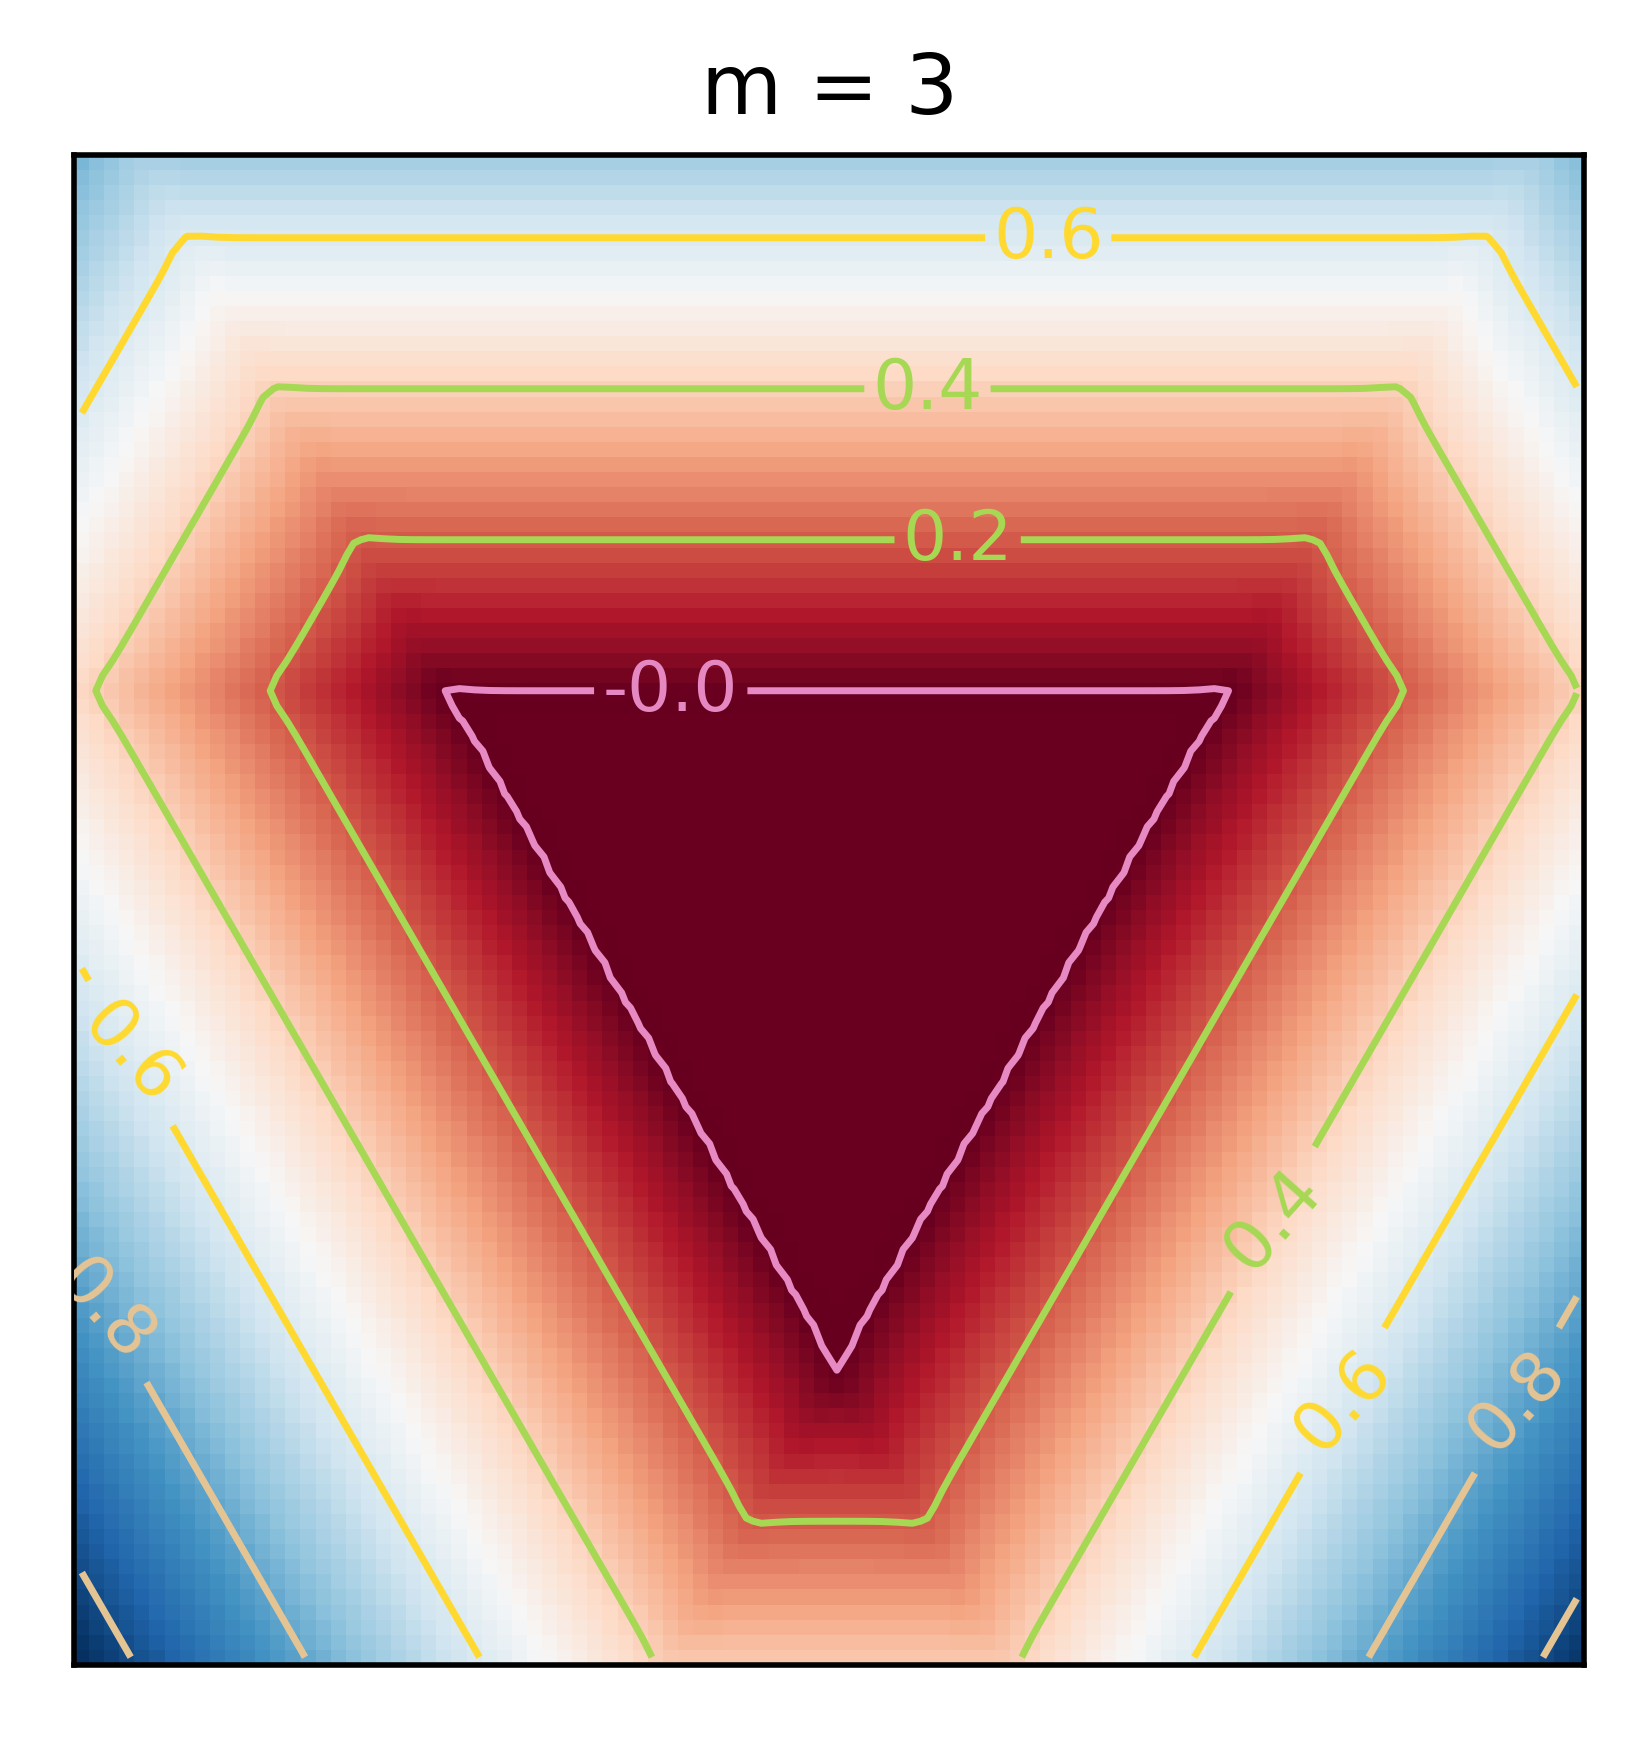
\includegraphics[scale=0.4]{truedist3.png}
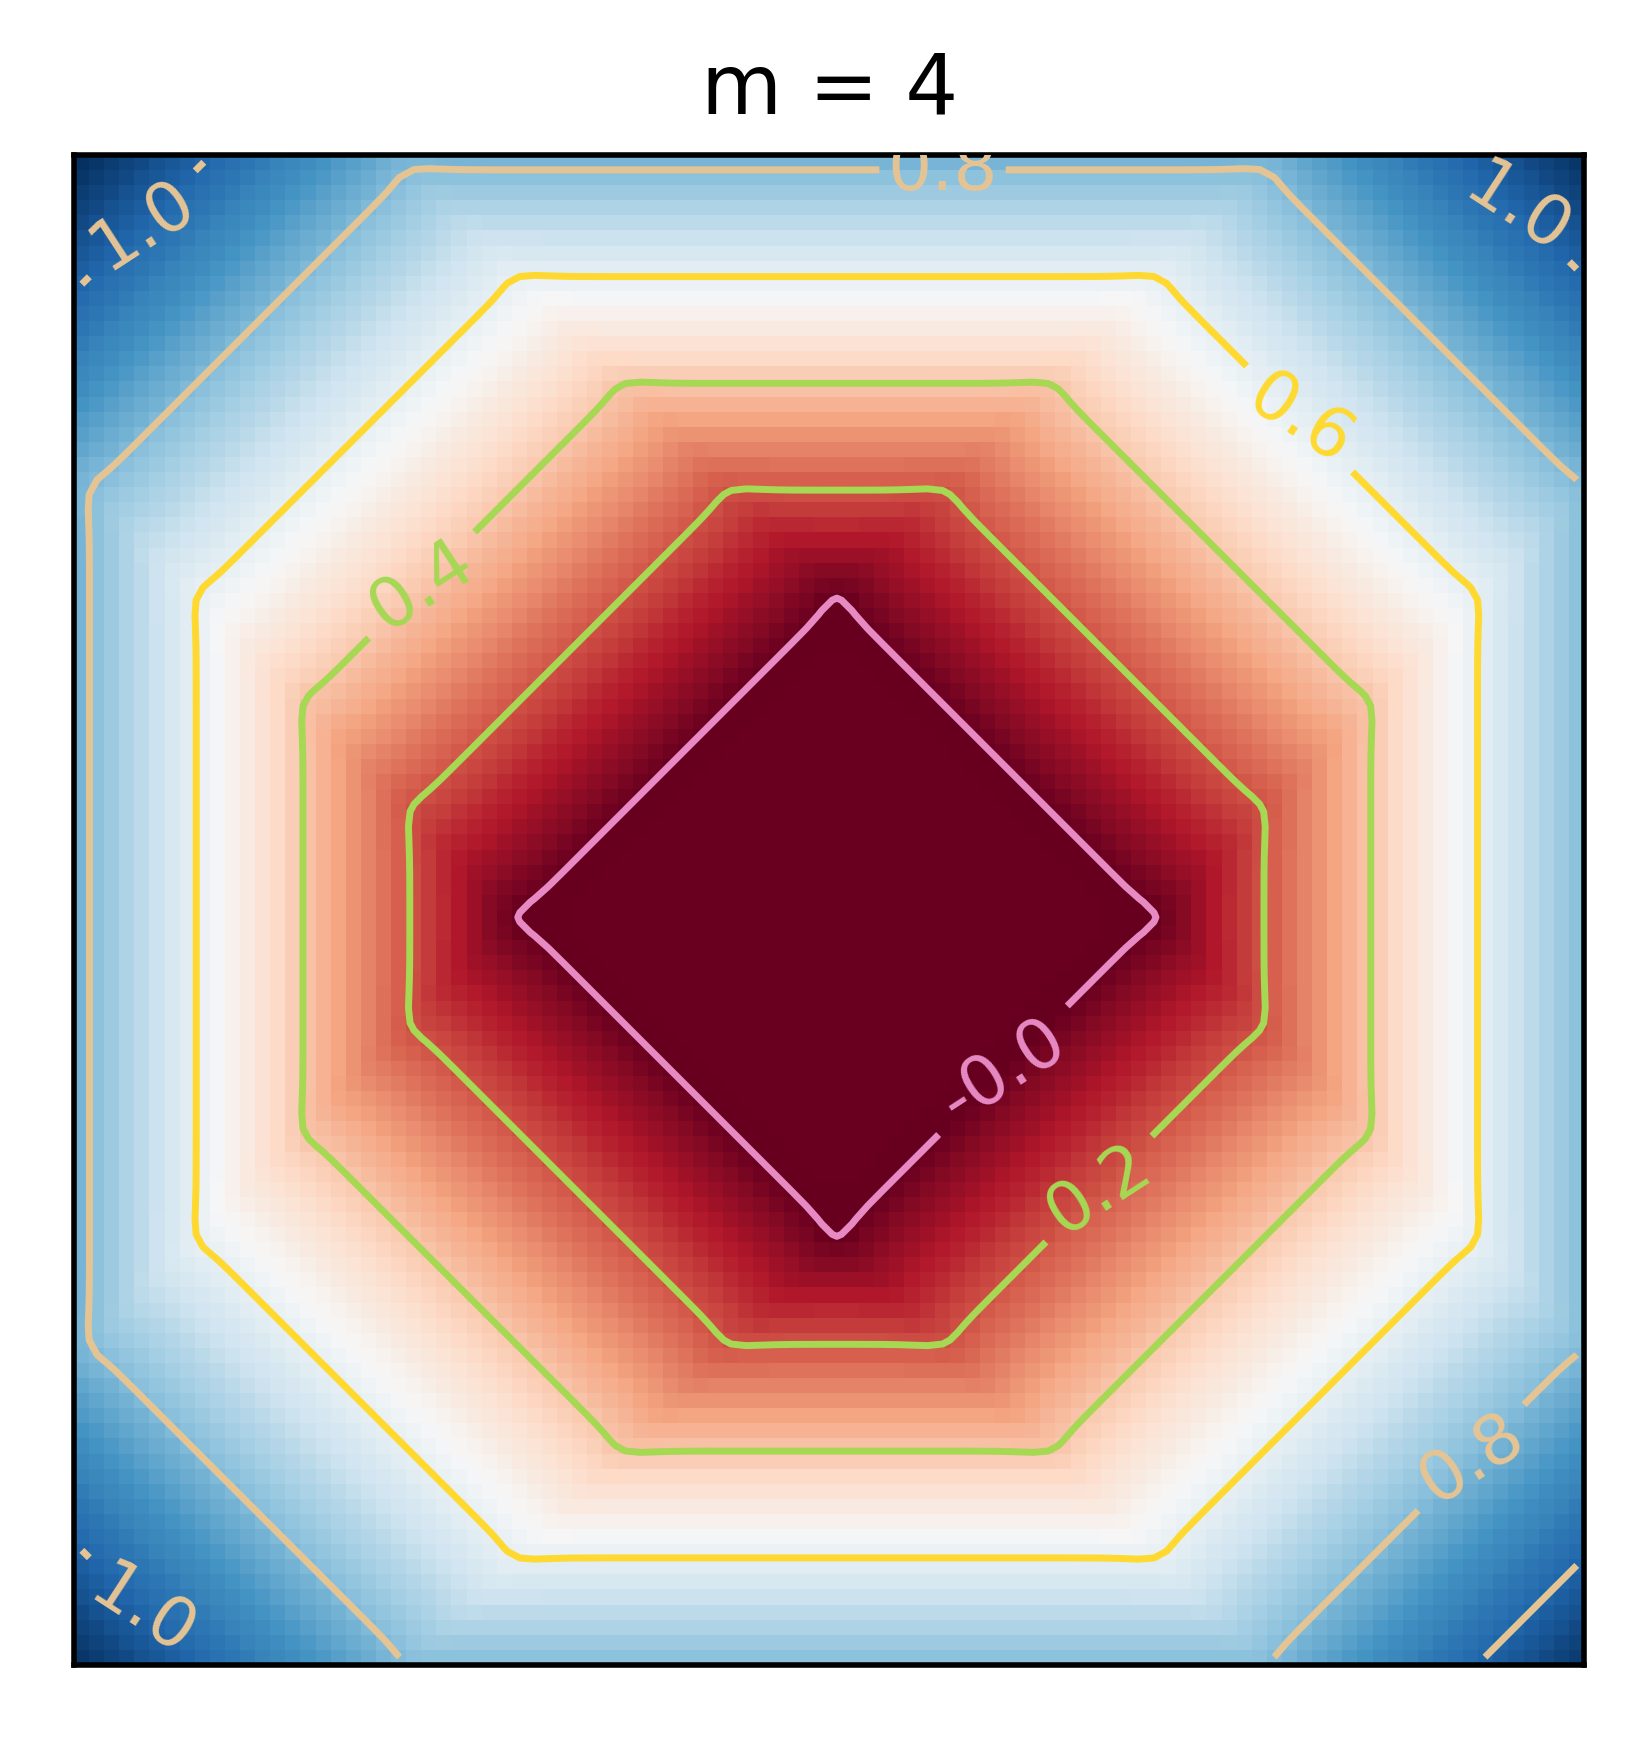
\includegraphics[scale=0.4]{truedist4.png}
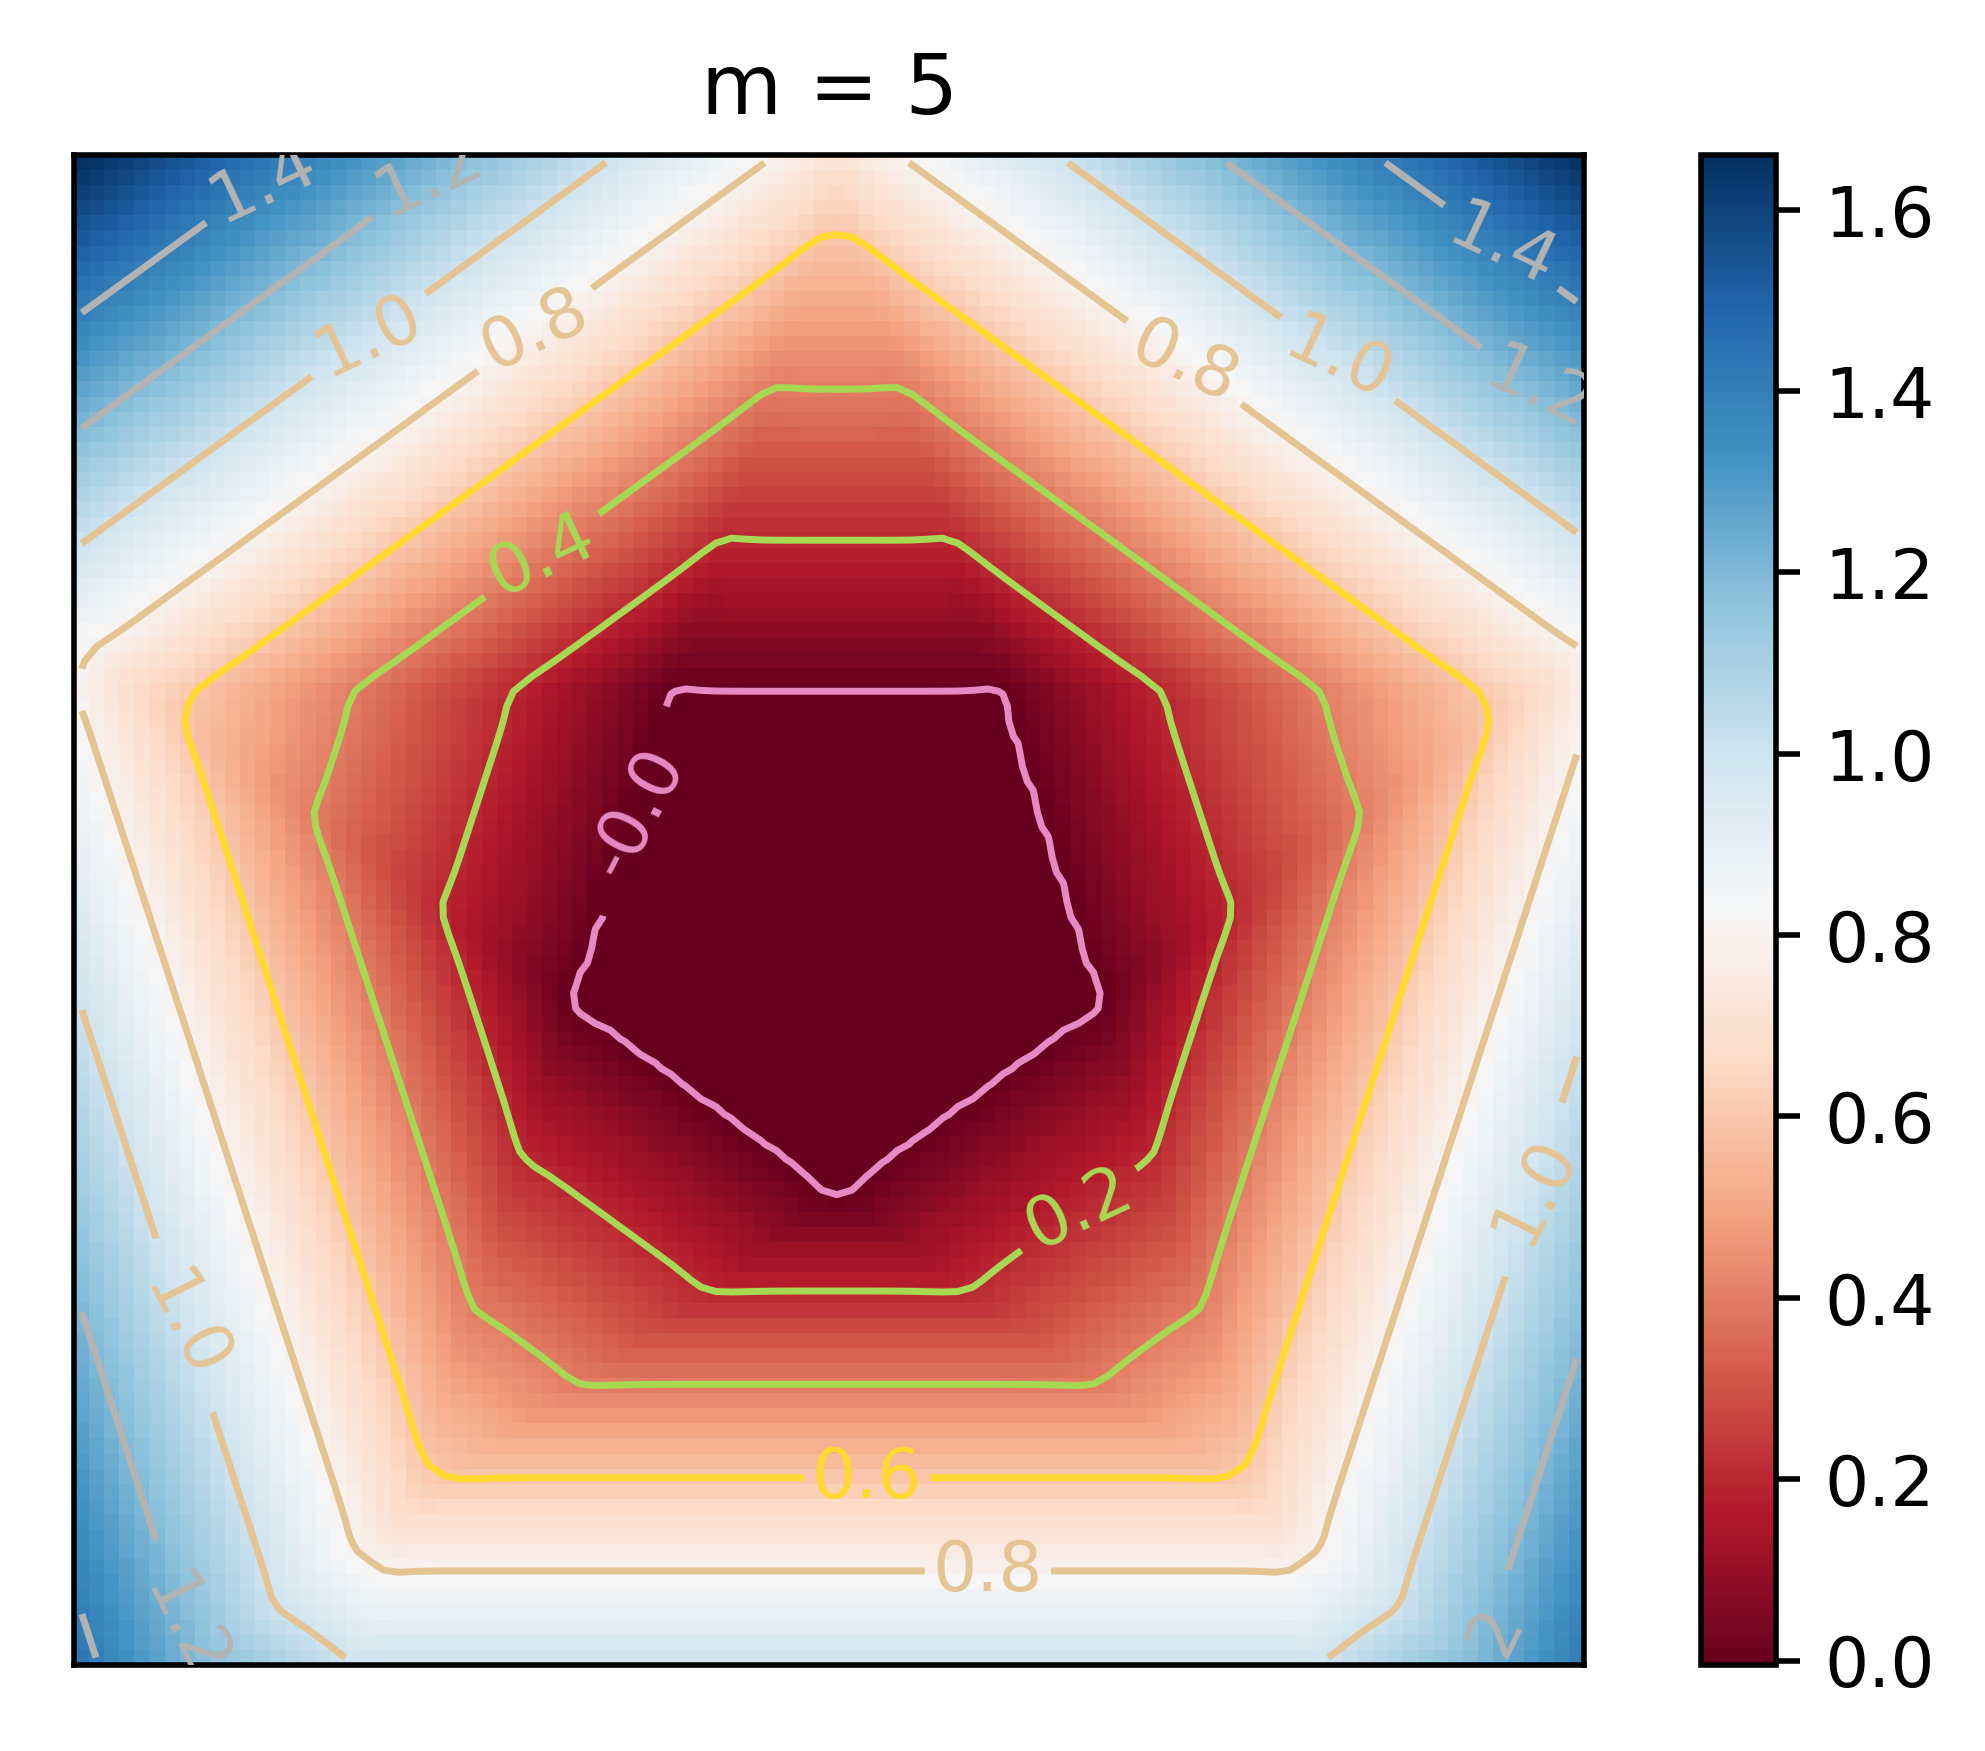
\includegraphics[scale=0.4]{truedist5.png}
\end{center}
\caption{Increasingly complicated true distributions $q_m(x,y)$ on $[-1,1]^2 \times \mathbb{R}$.}
\label{figure:simp_func_complex}
\end{figure}

\begin{table}[h]
    \begin{center}
    \begin{tabular}
    {r l l l l}
    \toprule
      \textbf{m}  & \textbf{Nonlinearity}  & \textbf{Mean} & \textbf{Std}\\ 
    \midrule
    3 & ReLU & 0.526301 & 0.027181\\
    3 & SiLU & 0.522393 & 0.026342\\
    4 & ReLU & 0.539590 & 0.024774\\
    4 & SiLU & 0.539387 & 0.020769\\
    5 & ReLU & 0.555303 & 0.002344\\
    5 & SiLU & 0.555630 & 0.021184\\
   \bottomrule
   \end{tabular}
    \end{center}
    \caption{\footnotesize RLCT estimates for ReLU and SiLU.}
    \label{table:hyper}
\end{table}

\begin{figure}[h]
\begin{center}
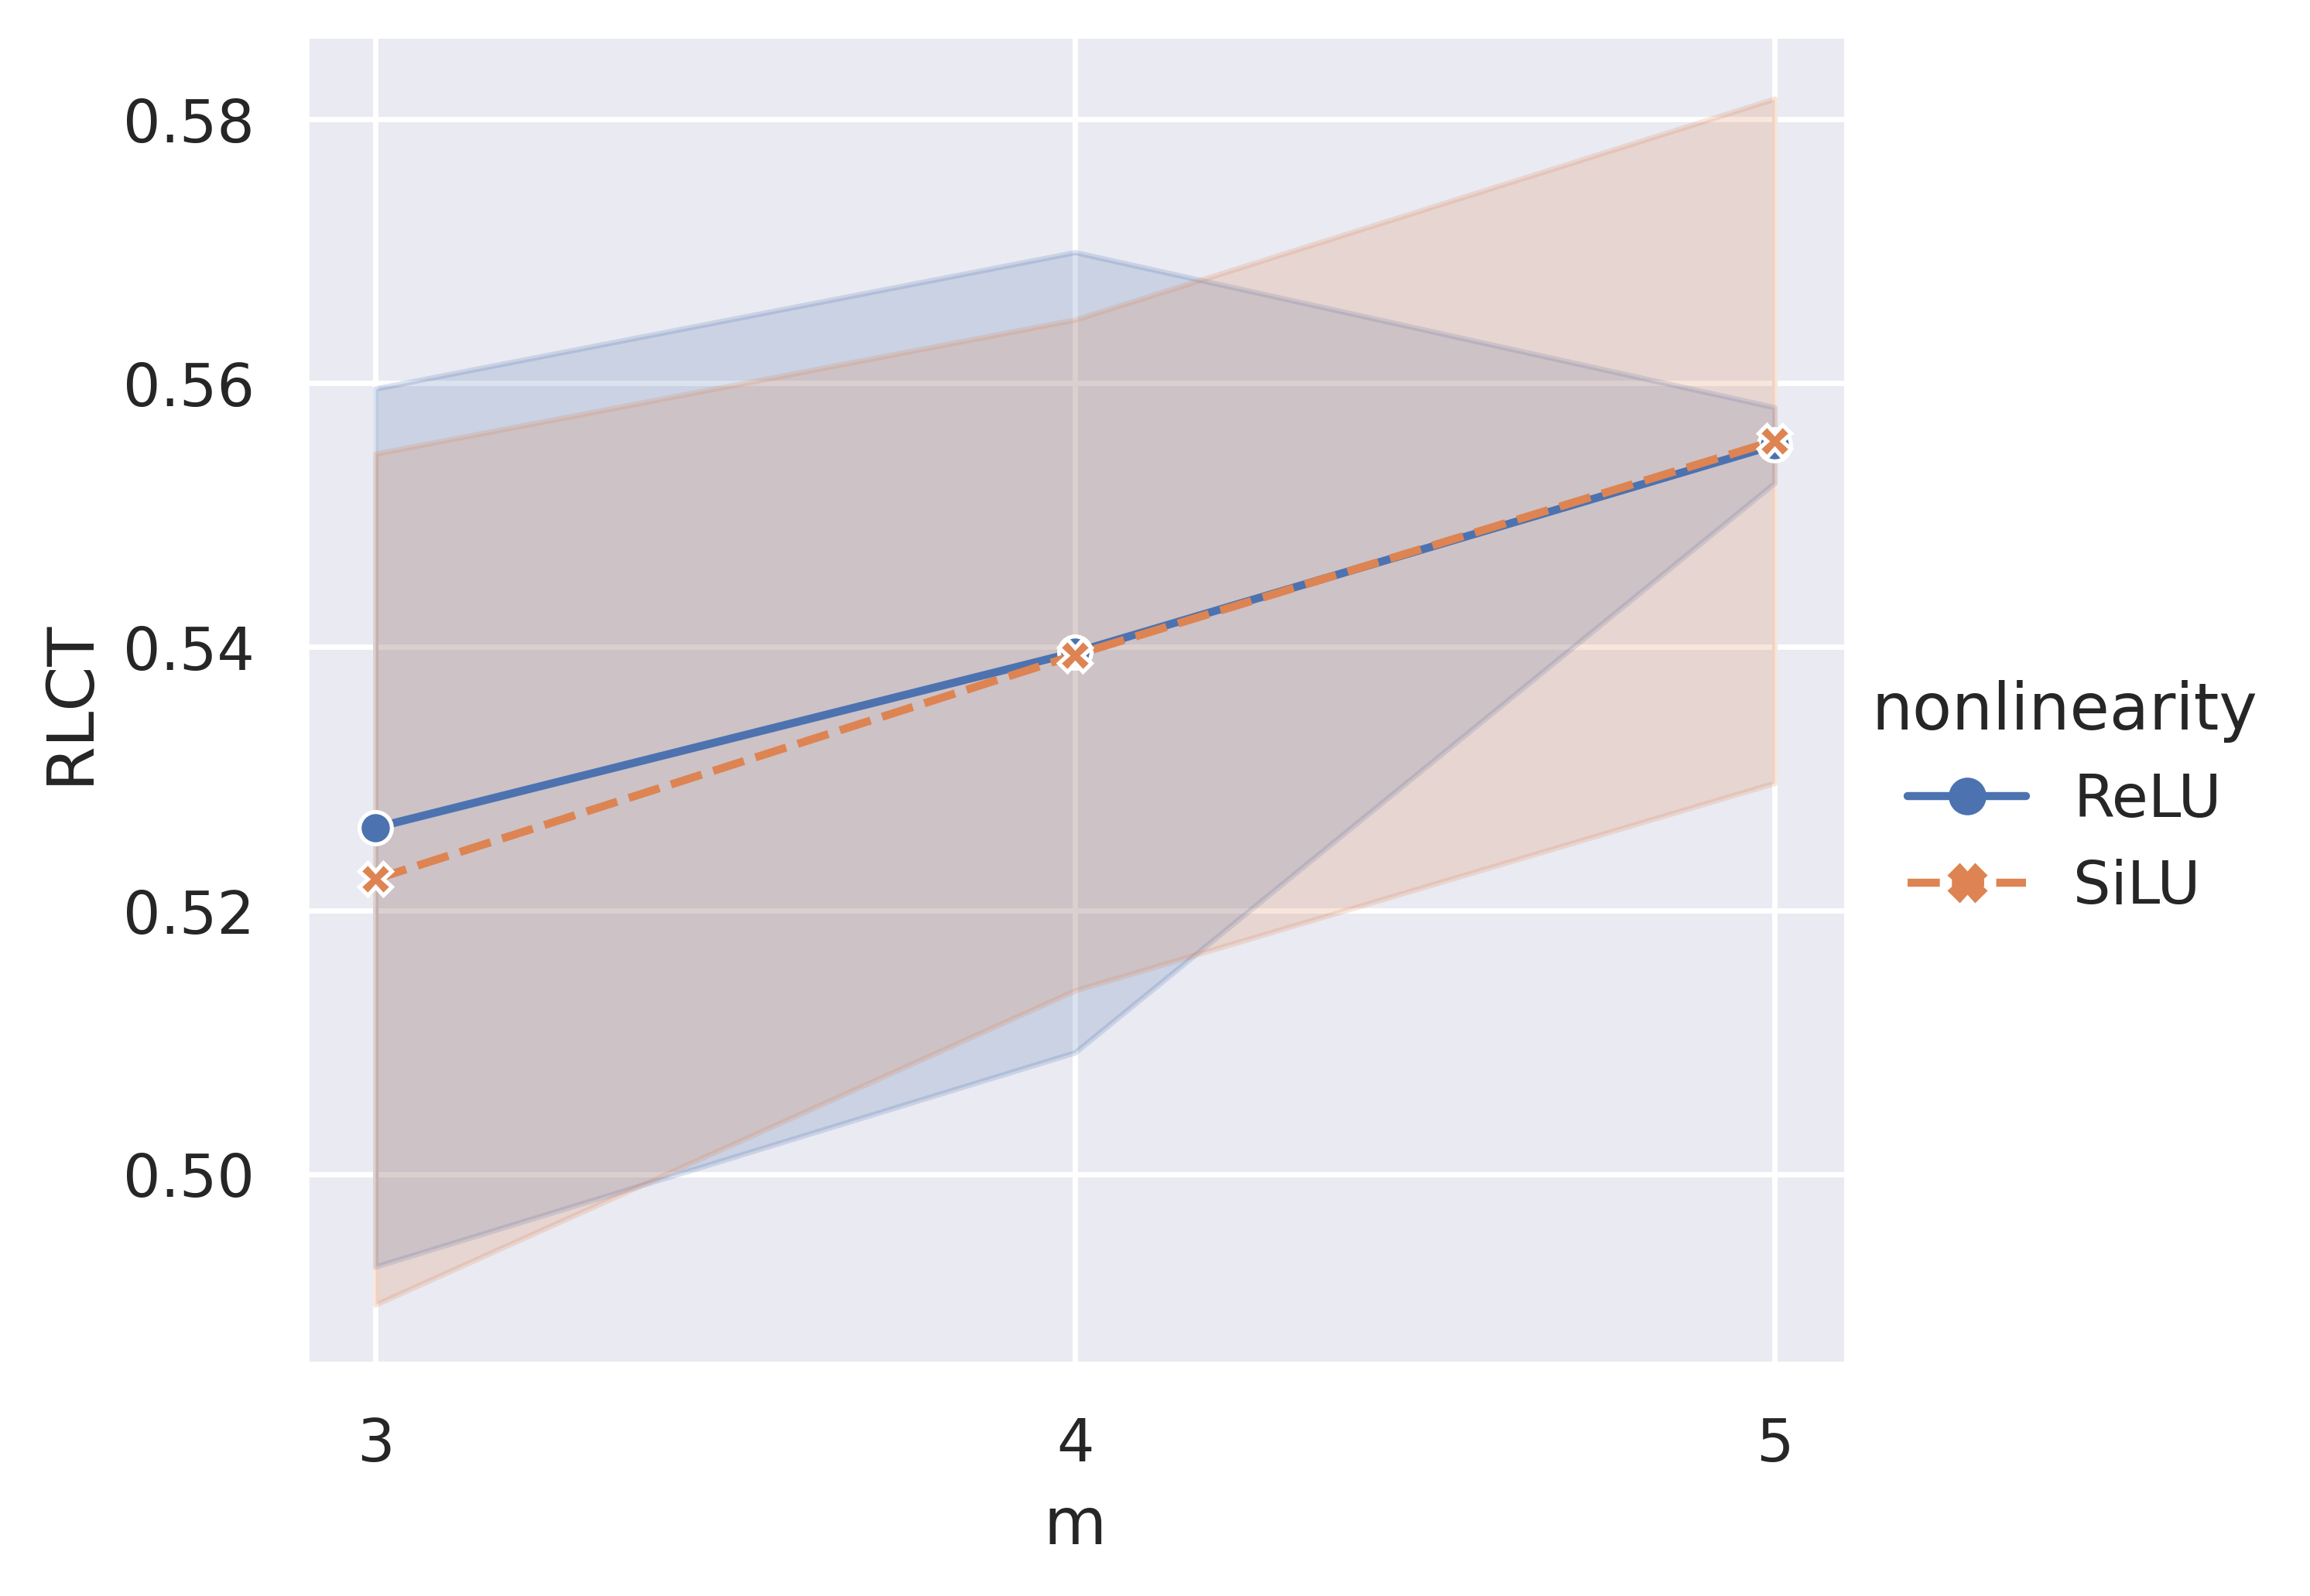
\includegraphics[scale=0.6]{RLCTplot.png}
\end{center}
\caption{RLCT estimates for ReLU and SiLU. Shaded region shows one standard deviation.}
\label{figure:simp_func_complex2}
\end{figure}

Given an integer $3 \le m \le H$ we define a network $\kappa_m \in W$ and $q_m(y|x) := p(y|x, \kappa_m)$ as follows. Let $g \in SO(2)$ stand for rotation by $\frac{2\pi}{m}$, set $w_1 = g^{\tfrac{1}{2}} e_1$ where $e_i$ denote unit vectors. The components of $\kappa_m$ are defined as follows: $w_i = g^{i-1} w_1$ for $1 \le i \le m$ and $w_i = 0$ for $i > m$, $b_i = - \tfrac{1}{3}$ and $q_i = 1$ for $1 \le i \le m$ and $b_i = q_i = 0$ for $i > m$, and finally $c = 0$ (the factor of $\tfrac{1}{3}$ ensures the relevant parts of the decision boundaries lie within $X = [-1,1]^2$) and the distribution $q_m$ is $\mathbb{Z}/m\mathbb{Z}$-invariant. We let $q(x)$ be the uniform distribution on $X$ and define $q_m(x,y) = q_m(y|x) q(x)$. Let $\varphi$ be a normal distribution $\mathcal{N}(0,50^2)$ centered on $W$ and consider the RLCTs of the triples $(p, q_m, \varphi)$. 

We conducted the experiments with $H = 5$, $n = 1000$. For each $m \in \{3,4,5\}$, Figure \ref{figure:simp_func_complex} shows the estimated RLCT where the error bars account for sampling variability\footnote{See ??? for code to reproduce this figure.}. Note that in all cases the number of parameters in $W$ is $d = 21$ and the RLCTs are less than 1\footnote{Not only are these models not regular, they are not even minimally singular since the dimension of the \emph{set} of true parameters, viewed as a submanifold, is $10$ when $m = 5$. Hence if this model were minimally singular the RLCT would have to be $11/2$}. Algorithm \ref{alg:thm4} in Appendix \ref{appendix:RLCT_estimation} details the estimation procedure for the RLCT which we base on \citep[Theorem 4]{watanabe_widely_2013}. 

The comments of \citep[\S 7.6]{watanabe_algebraic_2009} are based on the results of \citep[\S 7.2]{watanabe_algebraic_2009} which are summaries of \cite{??,??}. In \cite{??} the nonlinearity is the identity (reduced rank regression) and in \cite{??} the true distribution is always the zero function and the nonlinearity is $\operatorname{tanh}(x)$.

The RLCT estimates for the two-layer SiLU network (\ref{??}) provide evidence that this model is not minimally singular, when combined with the symmetric true distribution $q^{SiLU}_m(x,y)$. Starting from the weight vector of this true distribution, varying $c$ or any of the $b_i$ independently takes the model off the set of true parameters, so that the normal bundle has dimension $> H + 1$. Hence the RLCT in the minimally singular case would be bounded below by $3$ in the case $H = 5$, but our estimates for the RLCT are $< 0.6$.

We show in Appendix \ref{??} that when $m = H$ the set of true parameters $W_0 \subseteq W$ is a regular submanifold of dimension $m$. Hence if such a model is minimally singular its RLCT will be $\tfrac{1}{2}( (4m + 1) - m ) = \tfrac{1}{2}( 3m + 1 )$. In the case $m = 5$ we observe an RLCT more than an order of magnitude less than the value $8$ predicted by this formula.

\section{Future directions}
We claim that the RLCT is \textit{the} correct way to account for model complexity in a deep neural network. We do not however claim that the RLCT can be easily estimated for a deep neural network\footnote{Hironaka's resolution of singularities guarantees existence. But the proof is not constructive. It is notoriously difficult to do the so-called blowup transformations in high dimensions to obtain the standard form.}. The intractability of RLCT estimation may not in reality be a significant deterrent. For instance, used in the context of model selection, the exact value of the RLCT is not as important as model selection consistency, i.e., if using the estimated RLCT leads to the same model being selected as if the true RLCT were being used. 

For very few singular models have theoretical RLCTs been cataloged \citep{}. Theoretical RLCTs are certainly not known for modern deep neural networks where the network weights number on the order of $n$. Furthermore singular learning theory, as it stands, cannot be directly applied to neural networks with the ReLU activation function. 

At present there does not exist a method of sampling from the Bayesian posterior for large neural networks which is sufficiently accurate to yield accurate RLCT estimates. Variants of MCMC are the gold standard for such estimations, but these techniques do not scale to large networks; consequently we restrict to small networks (TODO: death of local RLCT idea?)


Despite this, we have  illustrated that it is still possible to reap the insights offered by singular learning theory. In particular we showed that being Bayesian in the final layers, though a pale substitute for the full Bayes predictive distribution, nonetheless demonstrates humble improvements over point estimators. 
%\subsubsection*{Author Contributions}
%If you'd like to, you may include  a section for author contributions as is done
%in many journals. This is optional and at the discretion of the authors.
%
%\subsubsection*{Acknowledgments}
%Use unnumbered third level headings for the acknowledgments. All
%acknowledgments, including those to funding agencies, go at the end of the paper.


\bibliography{iclr2021_conference}
\bibliographystyle{iclr2021_conference}

\appendix
\section{Appendix}

\subsection{RLCT estimation} \label{appendix:RLCT_estimation}

%From derivations in \citep{watanabe_widely_2013}, we can glean several useful asymptotic characterizations of the RLCT. To set this up, we begin with some definitions. 

Let $L_n(w)$ be the negative log likelihood as in \eqref{eq:nll}. Define the data likelihood at inverse temperature $\beta >0$ to be $p^\beta(\mathcal D_n | w) = \Pi_{i=1}^n p(y_i |x_i, w)^\beta$ which can also be written 
\begin{equation}
p^\beta(\mathcal D_n | w) = \exp(-\beta n L_n(w)).
\label{general_likelihood}
\end{equation}
The posterior distribution, at inverse temperature $\beta$, is defined as 
\begin{equation}
p^\beta(w|\mathcal D_n) = \frac{\Pi_{i=1}^n p(y_i|x_i,w)^\beta \varphi(w)}{\int_W \Pi_{i=1}^n p(y_i|x_i,w)^\beta \varphi(w)} = \frac{p^\beta(\mathcal D_n|w) \varphi(w)}{p^\beta(\mathcal D_n)}
\label{general_posterior}
\end{equation}
where $\varphi$ is the prior distribution on the network weights $w$ and
\begin{equation}
p^\beta(\mathcal D_n) = \int_W p^\beta(\mathcal D_n|w) \varphi(w) \,dw
\label{general_marginal_likelihood}
\end{equation}
is the marginal likelihood of the data at inverse temperature $\beta$. 
Finally, denote the expectation of a random variable $R(w)$ with respect to the tempered posterior $p^\beta(w|\mathcal D_n)$ as
\begin{equation}
{\E}_w^\beta [R(w)] = \int_W R(w) p^\beta(w|\mathcal D_n) \,dw
\label{general_expectation_posterior}
\end{equation}
% There are two senses to the estimation that is required of the real log canonical threshold. In the first sense, assuming the true distribution $q$ is known, we may be able to only approximate $\lambda(q)$. In the second sense, we must grapple with the fact that $q$ is not known and the plug-in procedure $\lambda(\hat q)$ is not sound. Works addressing the former vein largely come from researchers well-versed in algebraic geometry \cite{lin_ideal-theoretic_2017,imai_estimating_2019} while statisticians tend to treat the second estimation aspect \cite{drton_bayesian_2017}.

% There are two senses to the estimation that is required of the real log canonical threshold. In the first sense, assuming the true distribution $q$ is known, we may be able to only approximate $\lambda(q)$. In the second sense, we smut grapple with the fact that $q$ is not known and the plug-in procedure $\lambda(\hat q)$ is not sound. Works addressing the former vein largely come from researchers well-versed in algebraic geometry \cite{lin_ideal-theoretic_2017,imai_estimating_2019} while statisticians tend to treat the second estimation aspect \cite{drton_bayesian_2017}.
In the main text, we drop the superscript in the quantities \ref{general_likelihood}, \ref{general_posterior}, \ref{general_marginal_likelihood}, \ref{general_expectation_posterior} when $\beta = 1$, e.g., $p(\mathcal D_n)$ rather than $p^1(\mathcal D_n)$.


Assuming the conditions of Theorem 4 in \cite{watanabe_widely_2013} hold, we have
\begin{equation}
    {\E}_w^\beta [nL_n(w)] = nL_n(w_0) + \frac{\lambda }{\beta} + U_n \sqrt{\frac{\lambda}{2 \beta}} + O_p(1)
    \label{eq:Theorem4_WBIC}
\end{equation}
where $\beta_0$ is a positive constant and $U_n$ is a sequence of random variables satisfying ${\E}_n U_n = 0$. %Assuming $q(y|x)$ is realizable (which we do), $U_n$ behaves nicely ???insert some of those nice properties???.
In Algorithm \ref{alg:thm4}, we describe an estimation procedure for the RLCT based on the asymptotic result in \eqref{eq:Theorem4_WBIC}.
%To approximate the integral $E_w^\beta [n L_n(w)]$ on the left-hand-side of \eqref{eq:Theorem4_WBIC} we use NUTS. 
%However, the $p^\beta(w|\mathcal D_n)$ is intractable for any $\beta>0$, rendering computation of $E_w^\beta$ challenging. For regular models, the Laplace approximation to ${\E}_w^\beta [R(w)]$ would be reasonable (as guaranteed for instance by the Berstein-von Mises theorem.) Recall the Laplace approximation in this case would replace ${\E}_w^\beta$ with an expectation with respect to a normal random variable with mean $w_0$, which is a mode of $L_n$, and covariance which is the Hessian $H_{ij} =\frac{\partial^2 L_n}{\partial w_i \partial w_j}$. But as we discussed earlier, for strictly singular models, the Laplace approximation does not hold.

The \emph{a posteriori} distribution was approximated using the NUTS variant of Hamiltonian Monte Carlo \citep{hoffman2014no} where the first 1000 steps were omitted and $20,000$ samples were collected.  Each $\hat \lambda(\mathcal D_n)$ estimate in Algorithm \ref{alg:thm4} was performed by linear regression on the pairs $\{ (1/\beta_i, \mathbb{E}^{\beta_i}_w[ nL_n(w) ] ) \}_{i=1}^5$ where the five inverse temperatures $\beta_i$ are centered on high temperature $1/\log(20000)$.

\begin{algorithm}[tb]
	\caption{RLCT via Theorem 4}
	\label{alg:thm4}
	\begin{algorithmic}
		\STATE {\bfseries Input:} range of $\beta$'s, set of training sets $\mathcal T$ each of size $n$, approximate samples $\{w_1,\ldots,w_R\}$ from $p^\beta(w|\mathcal D_n)$ for each training set $\mathcal D_n$ and each $\beta$
		\FOR{training set $\mathcal D_n \in \mathcal T$}
    		\FOR{$\beta$ in range of $\beta$'s}
        		\STATE Approximate ${\E}_w^\beta [nL_n(w)]$ with $\frac{1}{R} \sum_{i=1}^R nL_n(w_r)$ where $w_1,\ldots,w_R$ are approximate samples from $p^\beta(w|\mathcal D_n)$
    		\ENDFOR
    		\STATE Perform generalized least squares to fit $\lambda$ in \eqref{eq:Theorem4_WBIC}, call result $\hat \lambda(\mathcal D_n)$
		\ENDFOR
		\STATE {\bfseries Output:} $\frac{1}{|\mathcal T|} \sum_{\mathcal D_n \in \mathcal T} \hat \lambda(\mathcal D_n)$
	\end{algorithmic}
\end{algorithm}



\subsection{Connection between RLCT and generalization} \label{appendix:generalization_theory}
For completeness, we sketch the derivation of \eqref{eq:RLCT_generalization} which gives the asymptotic expansion of the average generalization error ${\E}_n G(n)$ of the Bayes prediction distribution  in singular models. The exposition is an amalgamation of various works published by Sumio Watanabe, but is mostly based on the textbook \cite{watanabe_algebraic_2009}. 

To understand the connection between the RLCT and $G(n)$, we first define the so-called \textbf{Bayes free energy} as 
\[
F(n) = -\log p(\mathcal D_n)
\]
whose expectation admits the following asymptotic expansion \cite{watanabe_algebraic_2009}:
\[
{\E}_n F(n) =  {\E}_n n S_n + \lambda \log n + o(\log n)
\]
where $S_n = -\frac{1}{n} \sum_{i=1}^n \log q(y_i|x_i)$ is the entropy. 
%This deceptively simple result is actually based on a set of sophisticated tools, in particular Hironaka's resolution theorem from algebraic geometry.
The expected Bayesian generalization error is related to the Bayes free energy as follows
\[
{\E}_n G(n) = \E F(n+1) - \E(F_n)
\]
Then for the average generalization error, we have
\begin{equation}
{\E}_n G(n) = \lambda/n + o(1/n).
\label{eq:bayesgenerr}
\end{equation}
Since models with more complex singularities have smaller RLCTs, this would suggest that the more singular a model is, the better its generalization (assuming one uses the Bayesian predictive distribution for prediction). In this connection it is interesting to note that simpler (relative to the model) true distributions lead to more singular models (Section \ref{section:simple_func}).

That the RLCT has such a simple relationship to the Bayesian generalization error is remarkable. On the other hand, the practical implications of (\ref{eq:bayesgenerr}) are limited. This is because the Bayes predictive distribution in the case of a deep neural network is itself intractable. While we believe that approximations to the Bayesian predictive distribution, say via variational inference, might inherit a similar relationship between generalization and the (variational) RLCT, serious theoretical developments will be required to rigorously establish this. The challenge comes from the fact that for approximate Bayesian predictive distributions, the free energy and generalization error have different learning coefficients $\lambda$. This was well documented in the case of a neural network with one hidden layer \citep{nakajima_variational_2007}. 

\subsection{Details for generalization error experiments}
\label{appendix:generalizaton}

\textbf{Simulated data}
The distribution of $x \in \mathbb R^3$ is set to $q(x)=N(0,I_3)$. 
In the realizable case, $y \in \mathbb R^3$ is drawn according to $q(y|x) = p(y|x,\theta_0)$ as in \eqref{eq:genexp_model}. In the nonrealizable setting, we set $q(y|x) \propto \exp\{-|| y - h_{w_0}(x) ||^2/2\},$ where $w_0 = (A_0,B_0)$ is drawn according to the PyTorch model initialization of $h$.
%???mention $x_test_std$.???

%\textbf{Network architecture} In our experiments, $f = h \circ g$ where $g$ is a sequence of 
%\[
%\text{linear} \circ \text{ReLU} \circ \ldots \text{linear}
%\]
%and $h$ is either
%\begin{equation}
%    \text{linear} \circ \text{ReLU} \circ \text{linear} 
%    \label{eq:rr_with_relu}
%\end{equation}
%or
%\begin{equation}
%    \text{linear}  \circ \text{linear}. 
%    label{eq:rr_no_relu}
%\end{equation}
%We fix the number of hidden units in $g$, the feedforward ReLU block, to 5 and the number of hidden units in $h$, the last two years, to 3. We varied the number of layers in $g$ between $1$ and $5$.

\textbf{MAP training}
The MAP estimator is found via stochastic gradient descent using the mean-squared-error loss with minibatch set to ???. Training was set to 5000 epochs. No form of early stopping was employed.

\textbf{Calculating the generalization error}
Using a held-out-test set $T_{n'} = \{(x_i',y_i')\}_{i=1}^{n'}$, we calculate the average generalization error as
\begin{equation}
\frac{1}{n'} \sum_{i=1}^{n'} \log q(y_i'|x_i') - {\E}_n \frac{1}{n'} \sum_{i=1}^{n'} \log \hat q_n(y_i'|x_i')
\label{eq:computed_avgGn}
\end{equation}
Assume the held-out test set is large enough so that the difference between ${\E}_n G(n)$ and \eqref{eq:computed_avgGn} is negligible. We will refer to them interchangeably as the average generalization error. In our experiments we use $n' = 10,000$ and $30$ draws of the dataset $\mathcal{D}_n$ to estimate ${\E}_n$.

\textbf{Last layer(s) inference}
Without loss of generality, we discuss performing inference in the $w$ parameters of $h$ while freezing the parameters of $g$ at the MAP estimate. The steps easily extends to performing inference over the final layer only of $f = h \circ g$. Let $\tilde x_i = g_{v_{map}}(x_i)$. Define a new transformed dataset $\tilde{\mathcal D}_n = \{(\tilde x_i, y_i) \}_{i=1}^n$. We take the prior on $w$ to be standard Gaussian. 
Define the posterior over $w$ given $\tilde{\mathcal D}_n$ as:
\begin{equation}
p(w | \tilde{\mathcal D}_n) \propto p(\tilde{\mathcal D}_n | w) \varphi(w) = \Pi_{i=1}^n \exp\{-|| y_i - h_w(\tilde x_i) ||^2/2\} \varphi(w)
\label{eq:last_layer_posterior}
\end{equation}
Define the following approximation to the Bayesian predictive distribution
$$
\tilde p(y|x, \mathcal D_n) = \int p(y|x,(v_{map},w)) p(w|\tilde{\mathcal D}_n) \,dw.
$$
Let $w_1,\ldots,w_R$ be some approximate samples from $p(w | \tilde{\mathcal D}_n)$. Then we approximate $\tilde p(y|x, \mathcal D_n)$ with
\[
\frac{1}{R} \sum_{r=1}^R p(y|x,(v_{map},w_r))
\]
where $R$ is a large number, set to 1000 in our experiments. We consider the Laplace approximation and the NUTS variant of HMC for drawing samples from $p(w | \tilde{\mathcal D}_n)$:

\begin{itemize}
	\item \textbf{Laplace in the last layer(s)}
	Recall $\theta_{map} = (v_{map}, w_{map})$ is the MAP estimate for $f_\theta$ trained with the data $\mathcal D_n$. With the Laplace approximation, we draw $w_1,\ldots w_R$ from the Gaussian
	\[
	N(w_{map}, \Sigma)
	\]
	where $\Sigma = (- \nabla^2 \log p(w| \tilde{\mathcal D}_n) |_{w_{map}})^{-1}$ is the inverse Hessian\footnote{Following \citet{kristiadi_being_2020}, the code for the exact Hessian calculation is borrowed from \url{https://github.com/f-dangel/hbp}} of the negative log posterior evaluated at the MAP estimate of the mode.
	\item \textbf{MCMC in the last layer(s)}
	We used the NUTS variant of HMC to draw samples from \eqref{eq:last_layer_posterior} with the first 1000 samples  discarded.. Our implementation used the \texttt{pyro} package in \texttt{PyTorch}.
	
\end{itemize}



%We have to be careful when we speak of the generalization error of the approximate predictive distribution above. For a proper comparison to ${\E}_n G_{map}(n)$ or ${\E}_n G_{mle}(n)$, we have to look at 
%\begin{equation}
%{\E}_n G_{mcmcrr}(n) =  KL (q(y|x) || p_{mcmcrr}(y|x, \mathcal D_n) )
%\label{G_LLB}
%\end{equation}
%where ${\E}_n$ averages out the randomness of both $D_n$ and  $v_{map}$. 
%
%An alternative is to condition on $v_{map}$, using $g_{v_{map}}$ as a feature extractor in a preprocessing step. Then, assuming realizability $q(y|x) = p(y|x,(v_0,w_0))$ we may examine the generalizaton error
%\begin{equation}
%E_{\mathcal D_n | v_{map}} KL( p(y|x,(v_{map},w_0)) || p_{mcmcrr}(y|x, \mathcal D_n) )
%\label{G_LLB_vfixed}
%\end{equation}
%The average generalization error in \eqref{G_LLB_vfixed} is distinctly different from the one in \eqref{G_LLB}. The nice thing about \eqref{G_LLB_vfixed} is that we know its asymptotic expansion is $\lambda/n$ where $\lambda$ corresponds to the triplet $( p(y|x,(v_{map},w_0)), p(y| x, (v_{map},w)), \varphi(w))$. For certain functions $h_w$ where the true $\lambda$ is known, we can verify this in the experiments. (Not implemented yet).


\end{document}
